% Guia de implementacao do trabalho final (DAS5109): explicacao passo a passo,
% com equacoes, diagramas e os trechos reais do codigo MATLAB.
% Compilar:  cd guia && tectonic -X compile guia_implementacao.tex
\documentclass[11pt,a4paper]{article}

\usepackage{fontspec}
\usepackage[brazil]{babel}
\usepackage{microtype}
\usepackage[margin=2.2cm]{geometry}
\usepackage{amsmath,amssymb}
\usepackage{graphicx}
\usepackage{booktabs}
\usepackage{longtable}
\usepackage{tabularx}
\usepackage{array}
\usepackage{xcolor}
\usepackage[most]{tcolorbox}
\usepackage{listings}
\usepackage{tikz}
\usetikzlibrary{arrows.meta,positioning,shapes.geometric,fit,calc,backgrounds}
\usepackage[american]{circuitikz}
\usepackage{enumitem}
\usepackage{caption}
\usepackage{titlesec}
\usepackage{fancyhdr}
\usepackage{needspace}
\usepackage[hidelinks]{hyperref}

\graphicspath{{figs/}{../relatorio/figs/}}

\definecolor{azul}{HTML}{1F5FA8}
\definecolor{verde}{HTML}{2E8B57}
\definecolor{vermelho}{HTML}{D1495B}
\definecolor{amarelo}{HTML}{EDAE49}
\definecolor{cinza}{HTML}{555555}
\definecolor{roxo}{HTML}{6A4C93}

\titleformat{\section}{\Large\bfseries\color{azul}}{\thesection}{0.8em}{}
\titleformat{\subsection}{\large\bfseries\color{azul!80!black}}{\thesubsection}{0.7em}{}
\titleformat{\subsubsection}{\normalsize\bfseries}{\thesubsubsection}{0.6em}{}

\pagestyle{fancy}
\fancyhf{}
\fancyhead[L]{\small\color{cinza}DAS5109 -- Guia de implementa\c{c}\~ao do trabalho final}
\fancyhead[R]{\small\color{cinza}\thepage}
\renewcommand{\headrulewidth}{0.3pt}

\setlist{itemsep=2pt,topsep=4pt}
\setlength{\emergencystretch}{2em}
\captionsetup{font=small,labelfont=bf}

% ---------- caixas didaticas ----------
\newtcolorbox{intuicao}[1][]{enhanced,breakable,colback=verde!6,colframe=verde,
  fonttitle=\bfseries,title={Intui\c{c}\~ao#1},boxrule=0.6pt,arc=2pt,left=6pt,right=6pt}
\newtcolorbox{atencao}[1][]{enhanced,breakable,colback=vermelho!6,colframe=vermelho,
  fonttitle=\bfseries,title={Aten\c{c}\~ao#1},boxrule=0.6pt,arc=2pt,left=6pt,right=6pt}
\newtcolorbox{resumo}[1][]{enhanced,breakable,colback=azul!5,colframe=azul,
  fonttitle=\bfseries,title={Em resumo#1},boxrule=0.6pt,arc=2pt,left=6pt,right=6pt}
\newtcolorbox{logica}[1][]{enhanced,breakable,colback=roxo!6,colframe=roxo,
  fonttitle=\bfseries,title={L\'ogica passo a passo#1},boxrule=0.6pt,arc=2pt,left=6pt,right=6pt}
\newtcolorbox{resultado}[1][]{enhanced,breakable,colback=amarelo!10,colframe=amarelo!80!black,
  fonttitle=\bfseries,title={Resultado#1},boxrule=0.6pt,arc=2pt,left=6pt,right=6pt}

% ---------- codigo MATLAB ----------
\lstdefinestyle{matlabcod}{
  language=Matlab,
  basicstyle=\ttfamily\scriptsize,
  keywordstyle=\color{azul}\bfseries,
  commentstyle=\color{verde!60!black}\itshape,
  stringstyle=\color{vermelho},
  numbers=left, numberstyle=\tiny\color{cinza}, numbersep=6pt,
  frame=single, rulecolor=\color{cinza!50},
  breaklines=true, breakatwhitespace=false,
  postbreak=\mbox{\textcolor{cinza}{$\hookrightarrow$}\space},
  columns=fullflexible, keepspaces=true, showstringspaces=false,
  xleftmargin=14pt, aboveskip=6pt, belowskip=4pt}
\lstset{style=matlabcod}

% \codigo{arquivo}{primeira}{ultima}{legenda}{rotulo}: trecho real do arquivo
\newcommand{\codigo}[5]{%
  \lstinputlisting[style=matlabcod,linerange={#2-#3},firstnumber=#2,label={#5},
    caption={\texttt{\detokenize{#1}}, linhas #2 a #3: #4}]{../matlab/#1}}
% \codigointeiro{arquivo}{legenda}{rotulo}: arquivo inteiro
\newcommand{\codigointeiro}[3]{%
  \lstinputlisting[style=matlabcod,label={#3},
    caption={\texttt{\detokenize{#1}}: #2}]{../matlab/#1}}
\renewcommand{\lstlistingname}{C\'odigo}
\captionsetup[lstlisting]{font=small,labelfont=bf,singlelinecheck=false}

% nome de arquivo/funcao no texto
\usepackage{url}
\urlstyle{tt}
\makeatletter\def\UrlBreaks{\do\/\do\_\do\.\do\-}\makeatother
\newcommand{\arq}[1]{\path{#1}}

% ---------- notacao ----------
\newcommand{\Ipv}{I_{\mathrm{pv}}}
\newcommand{\Vt}{V_{\mathrm{t}}}
\newcommand{\vpv}{v_{\mathrm{pv}}}
\newcommand{\ipv}{i_{\mathrm{pv}}}
\newcommand{\Vbat}{V_{\mathrm{bat}}}
\newcommand{\Vref}{V_{\mathrm{ref}}}
\newcommand{\Ta}{T_{\mathrm{a}}}
\newcommand{\Voc}{V_{\mathrm{oc}}}
\newcommand{\Isc}{I_{\mathrm{sc}}}
\newcommand{\Vmp}{V_{\mathrm{mp}}}
\newcommand{\Imp}{I_{\mathrm{mp}}}

% ---------- estilos TikZ ----------
\tikzset{
  bloco/.style={draw=cinza,rounded corners=3pt,thick,align=center,font=\small,
                minimum height=1.25cm,minimum width=2.9cm,inner sep=4pt},
  ctrl/.style={bloco,draw=azul,fill=azul!10,very thick},
  dest/.style={bloco,draw=verde!70!black,fill=verde!8},
  aviso/.style={bloco,draw=vermelho,fill=vermelho!8},
  seta/.style={-{Stealth[length=2.6mm]},thick,draw=cinza},
  rot/.style={font=\scriptsize,color=cinza,inner sep=1.5pt}}

\title{\textbf{Guia de implementa\c{c}\~ao do trabalho final}\\[4pt]
  \large Energia fotovoltaica sob sombreamento parcial: painel, conversor, controle e MPPT\\[2pt]
  \normalsize DAS5109 -- Modelagem e Simula\c{c}\~ao de Processos (UFSC)}
\author{Explica\c{c}\~ao passo a passo, com equa\c{c}\~oes, diagramas e o c\'odigo MATLAB real}
\date{10 de novembro de 2026}

\begin{document}
\maketitle
\thispagestyle{fancy}

\begin{abstract}\noindent
Este guia explica, na ordem em que foi constru\'ido, tudo o que foi feito no trabalho final:
do modelo el\'etrico do painel at\'e a compara\c{c}\~ao de algoritmos de rastreamento do ponto de
m\'axima pot\^encia (MPPT) num dia real. Cada cap\'itulo traz a f\'isica, as equa\c{c}\~oes, os
diagramas e os trechos de c\'odigo que as implementam, com a l\'ogica explicada passo a passo.
Os trechos de c\'odigo s\~ao lidos diretamente dos arquivos de \texttt{matlab/} (n\~ao s\~ao
c\'opias digitadas), ent\~ao o que est\'a aqui \'e o que roda. Os n\'umeros v\^em dos arquivos de
\texttt{resultados/}.
\end{abstract}

\begin{tcolorbox}[colback=azul!5,colframe=azul,boxrule=0.6pt,arc=2pt,title={Como usar este guia}]
Cada cap\'itulo segue o mesmo roteiro: \textbf{(1)} o problema e a intui\c{c}\~ao f\'isica;
\textbf{(2)} as equa\c{c}\~oes; \textbf{(3)} um diagrama; \textbf{(4)} o c\'odigo, com uma caixa
\emph{L\'ogica passo a passo} que explica linha a linha o que ele faz; \textbf{(5)} os resultados.
As caixas coloridas t\^em papel fixo: verde = intui\c{c}\~ao, roxa = l\'ogica do c\'odigo,
vermelha = aten\c{c}\~ao (uma armadilha ou limita\c{c}\~ao), amarela = resultado num\'erico,
azul = resumo. Os coment\'arios dentro do c\'odigo est\~ao sem acentos, como nos arquivos
originais.
\end{tcolorbox}

\tableofcontents
\listoffigures

\clearpage
\section{Vis\~ao geral}\label{sec:visao}

O trabalho mede quanto de energia um painel fotovoltaico real perde quando uma parte dele
fica na sombra e o algoritmo de rastreamento (MPPT) \'e simples, e quanto um algoritmo global
recupera. Tudo foi feito em MATLAB (com a Optimization Toolbox s\'o para o \texttt{fsolve}), com c\'odigo escrito para ser lido por
um j\'unior (laços e nomes claros, coment\'arios sobre a f\'isica).

\subsection{A pergunta central}

\begin{resumo}
\textbf{Quanta energia o P\&O deixa de captar sob sombreamento parcial, e quanto um MPPT
global (PSO) recupera, considerando o aquecimento do painel e as perdas do conversor?}
\end{resumo}

A \'ultima parte da pergunta \'e o diferencial. Muitos estudos comparam MPPT com o painel a
temperatura fixa e um conversor ideal. Aqui o painel esquenta durante o dia e o conversor tem
perdas; o relat\'orio mede quanto isso muda a resposta.

\subsection{Por que sombra parcial \'e dif\'icil}

Um m\'odulo \'e uma fileira de c\'elulas em s\'erie, dividida em grupos chamados
\emph{subm\'odulos}. Cada subm\'odulo tem um \emph{diodo de bypass} em antiparalelo. Num
circuito em s\'erie todos conduzem a mesma corrente. Quando um subm\'odulo recebe menos luz, ele
n\~ao consegue gerar essa corrente; o diodo de bypass ent\~ao desvia a corrente em volta dele e
o subm\'odulo deixa de contribuir com tens\~ao.

O efeito \'e que a curva pot\^encia $\times$ tens\~ao deixa de ter um \'unico pico e passa a ter
\textbf{v\'arios picos}, um para cada combina\c{c}\~ao de subm\'odulos ``ligados''. Um algoritmo
local, como o P\&O (Perturba e Observa), sobe a ladeira do pico mais pr\'oximo e pode ficar preso
num pico local, mais baixo que o global. Um algoritmo global, como o PSO (Otimiza\c{c}\~ao por
Enxame de Part\'iculas), explora a curva inteira.

\subsection{O sistema modelado}\label{sec:diagrama_sistema}

O sistema tem quatro blocos em cadeia (cen\'ario $\to$ painel $\to$ conversor $\to$ bateria), um
modelo t\'ermico que acopla a temperatura ao painel, e dois la\c{c}os de controle. O la\c{c}o
\textbf{interno} (PI) mede a tens\~ao do painel $\vpv$ e ajusta a raz\~ao c\'iclica $d$ do conversor
para que $\vpv$ siga uma refer\^encia $\Vref$. O la\c{c}o \textbf{externo} (MPPT), mais lento, mede
tens\~ao e corrente m\'edias a cada per\'iodo $\Ta$ e escolhe uma nova $\Vref$. Um \emph{or\'aculo}
calcula o m\'aximo global verdadeiro, s\'o para medir a efici\^encia dos algoritmos.

\begin{figure}[htbp]
\centering
\begin{tikzpicture}[x=1cm,y=1cm]
  \node[bloco] (cen) at (0,0)    {\textbf{Cen\'ario}\\[-1pt]{\scriptsize $G$ por subm\'odulo,}\\{\scriptsize $T_{amb}$, vento}};
  \node[bloco] (pai) at (4.2,0)  {\textbf{Painel}\\[-1pt]{\scriptsize 3 subm\'odulos,}\\{\scriptsize bypass, 2 diodos}};
  \node[bloco] (con) at (8.4,0)  {\textbf{Buck-boost}\\[-1pt]{\scriptsize modelo m\'edio}\\{\scriptsize com perdas}};
  \node[bloco] (bat) at (12.6,0) {\textbf{Bateria}\\[-1pt]{\scriptsize 12\,V ideal}};
  \node[ctrl]  (mpp) at (4.2,2.9) {\textbf{MPPT}\\[-1pt]{\scriptsize P\&O, InC ou PSO}\\{\scriptsize a cada $\Ta=31$\,ms}};
  \node[ctrl]  (pi)  at (8.4,2.9) {\textbf{PI de tens\~ao}\\[-1pt]{\scriptsize $e=\vpv-\Vref$}\\{\scriptsize $d=K_p(e+\xi/T_i)$}};
  \node[bloco] (ter) at (4.2,-2.9) {\textbf{T\'ermico}\\[-1pt]{\scriptsize balan\c{c}o de energia}\\{\scriptsize calibrado no NMOT}};
  \node[bloco] (ora) at (8.4,-2.9) {\textbf{Or\'aculo}\\[-1pt]{\scriptsize m\'aximo global $P_g$}\\{\scriptsize $\eta=E/E_g$}};
  \draw[seta] (cen) -- node[rot,above]{$G$} (pai);
  \draw[seta] (pai) -- node[rot,above]{$\vpv,\ipv$} (con);
  \draw[seta] (con) -- node[rot,above]{$P_{out}$} (bat);
  \draw[seta] (cen.south) |- node[rot,above,pos=0.75]{$G,T_{amb},v$} (ter.west);
  \draw[seta] ([xshift=-6pt]ter.north) -- node[rot,left]{$T$} ([xshift=-6pt]pai.south);
  \draw[seta] ([xshift=6pt]pai.south) -- node[rot,right]{$P_{el}$} ([xshift=6pt]ter.north);
  \draw[seta] (ter) -- node[rot,above]{$T$} (ora);
  \draw[seta] (pai.north) -- node[rot,right]{$V,I$} (mpp.south);
  \draw[seta] (mpp) -- node[rot,above]{$\Vref$} (pi);
  \draw[seta] (pi.south) -- node[rot,right]{$d$} (con.north);
  \node[rot,anchor=west,text width=3.6cm] at (11.1,-2.9)
       {Em azul: o controle (MPPT e PI). O or\'aculo s\'o mede, n\~ao controla.};
\end{tikzpicture}
\caption{Fluxo do sistema. Cada seta \'e uma vari\'avel trocada entre blocos. Os dois la\c{c}os
de controle est\~ao em azul.}
\label{fig:sistema}
\end{figure}

\begin{intuicao}
Pense no PI como o motorista que mant\'em o carro na velocidade pedida (a tens\~ao $\Vref$), e no
MPPT como o passageiro que, de tempos em tempos, diz ``tente ir um pouco mais r\'apido''
(muda $\Vref$) e observa se a viagem rende mais. O passageiro s\'o pode falar depois que o
motorista j\'a estabilizou a velocidade, sen\~ao n\~ao consegue saber o efeito do pedido. Esse
\'e o crit\'erio de Femia (Cap\'itulo~\ref{sec:controle}), que fixa $\Ta$.
\end{intuicao}

\subsection{Mapa do reposit\'orio}

\begin{center}\small
\begin{tabularx}{\textwidth}{@{}l X c@{}}
\toprule
Pasta & O que cont\'em & Cap. \\
\midrule
\arq{matlab/painel}      & Modelo de 2 diodos, extra\c{c}\~ao de par\^ametros, sombreamento, valida\c{c}\~ao & 3, 4, 5 \\
\arq{matlab/termico}     & Balan\c{c}o t\'ermico e calibra\c{c}\~ao pelo NMOT & 6 \\
\arq{matlab/conversor}   & Buck-boost: ideal, m\'edio com perdas, chaveado, equil\'ibrio, CCM/DCM & 7 \\
\arq{matlab/controle}    & Lineariza\c{c}\~ao, resposta em frequ\^encia, margens, projeto do PI & 8 \\
\arq{matlab/mppt}        & P\&O, InC, PSO, duty fixo, rastreamento est\'atico & 9 \\
\arq{matlab/simulacao}   & Simula\c{c}\~ao din\^amica, quase-est\'atica, or\'aculo & 10 \\
\arq{matlab/cenarios}    & Perfil EN 50530, dia do PVGIS, sombras & 11 \\
\arq{matlab/experimentos}& \arq{exp01} a \arq{exp08}, que geram \arq{resultados/} e as figuras & 12 \\
\arq{matlab/tests}       & Testes automatizados (80) & 13 \\
\arq{relatorio/}, \arq{proposta/}, \arq{guia/} & Documentos em \LaTeX & --- \\
\bottomrule
\end{tabularx}
\end{center}

\subsection{Ordem de constru\c{c}\~ao}

O plano (\arq{docs/superpowers/plans/2026-10-27-trabalho-final-pv-mppt.md}) tem 16 tarefas
(0 a 15). Cada bloco s\'o foi constru\'ido depois que o anterior estava testado:

\begin{enumerate}
\item Reorganiza\c{c}\~ao do c\'odigo e harness de testes (tarefa 0).
\item Depend\^encia da c\'elula com $G$ e $T$ e KCL do m\'odulo (tarefa 1).
\item Extra\c{c}\~ao de par\^ametros, validada no KC200GT (tarefa 2).
\item Painel real ZTP-160M e sua valida\c{c}\~ao (tarefa 3).
\item Modelo t\'ermico (tarefa 4).
\item Conversor: modelo m\'edio, equil\'ibrio, CCM/DCM (tarefa 5) e modelo chaveado (tarefa 6).
\item Lineariza\c{c}\~ao e resposta em frequ\^encia (tarefa 7) e projeto do PI (tarefa 8).
\item Algoritmos de MPPT (tarefa 9).
\item Simula\c{c}\~ao din\^amica (tarefa 10) e quase-est\'atica (tarefa 11).
\item Cen\'arios (tarefa 12) e experimentos de resultados (tarefa 13).
\item Relat\'orio (tarefa 14) e revis\~ao final com publica\c{c}\~ao (tarefa 15).
\end{enumerate}

Depois veio uma etapa extra de \textbf{simplifica\c{c}\~ao do c\'odigo} (Cap\'itulo~\ref{sec:testes}).

\section{Decis\~oes de projeto (D1 a D17)}\label{sec:decisoes}

O plano registra 17 decis\~oes. As dez primeiras foram tomadas em 03/11/2026, ao validar o plano.
As demais surgiram durante a implementa\c{c}\~ao, quando um teste ou experimento mostrou que a
ideia inicial n\~ao funcionava. Entender o \emph{porqu\^e} de cada uma \'e o que permite defender
o trabalho.

{\small
\begin{longtable}{@{}p{0.7cm}p{2.5cm}p{5.6cm}p{6.6cm}@{}}
\toprule
\# & Tema & Decis\~ao & Por qu\^e \\ \midrule \endhead
D1 & Painel & ZTROON ZTP-160M; o KC200GT fica s\'o como benchmark da extra\c{c}\~ao
  & Valida o m\'etodo contra um resultado publicado (Villalva, 2009) e aplica ao painel real \\
D2 & Ferramentas & MATLAB base; depois, tamb\'em a Optimization Toolbox s\'o para o \texttt{fsolve} & Inicialmente sem toolboxes (LM pr\'oprio). Revisto em 10/11/2026: o \texttt{fsolve} em $\log_{10}$ de $R_s$ e $R_p$ d\'a os mesmos par\^ametros \\
D3 & Bateria & 12\,V constante (fonte ideal)
  & Sem sombra $V_{mp}\approx19{,}6$\,V $>12$\,V: o conversor abaixa. Com sombra o pico global cai para 7 a 13\,V: precisa elevar. O buck-boost \'e necess\'ario justamente para o MPPT global \\
D4 & Conversor & $f_s=20$\,kHz, $L\approx57\,\mu$H, $C\approx1{,}3$\,mF, perdas de cat\'alogo
  & 20\,kHz \'e inaud\'ivel e tem perdas de chaveamento pequenas nessa pot\^encia (o trabalho anterior usou 2\,kHz, com indutor 10 vezes maior) \\
D5 & EN 50530 & Tabelas B.2 a B.4 transcritas de um relat\'orio de ensaio T\"UV Rheinland
  & O texto da norma \'e pago; os valores conferem com as dura\c{c}\~oes impressas \\
D6 & Dia real & PVGIS hor\'ario de Florian\'opolis, com nuvens e sombra de poste sint\'eticas e declaradas
  & Dados hor\'arios n\~ao t\^em transit\'orios r\'apidos \\
D7 & Relat\'orio & \LaTeX, estilo do trabalho anterior & Continuidade com a disciplina \\
D8 & Valida\c{c}\~ao do painel & Sem curvas I-V (o datasheet n\~ao tem): STC, coeficiente t\'ermico de $P_{max}$, NMOT e KC200GT
  & Usa s\'o informa\c{c}\~ao publicada e declara a limita\c{c}\~ao \\
D9 & 2 diodos & Conven\c{c}\~ao de Ishaque: $a_1=1$, $a_2=1{,}2$, $I_{01}=I_{02}$; lei t\'ermica efetiva com $E_g$ ajustado pelo $K_v$
  & Com $E_g=1{,}12$\,eV o modelo d\'a $K_v=-0{,}106$\,V/K contra $-0{,}123$ medido; e o datasheet n\~ao identifica $I_{02}$ \\
D10 & $R_p$ & $R_p(G)=R_{p,ref}\,G_n/G$ (De Soto)
  & Com $R_p$ constante o ajuste previa perda de 26\,\% em 200\,W/m$^2$, contra 3 a 5\,\% t\'ipicos \\
D11 & T\'ermico & Convec\c{c}\~ao de Watmuff, radia\c{c}\~ao frente$\to$c\'eu e verso$\to$solo, capacidade pela massa do datasheet
  & McAdams j\'a inclui radia\c{c}\~ao e a contava duas vezes. Com as corre\c{c}\~oes: $k_h=0{,}79$ e $\tau\approx7$\,min \\
D12 & Projeto do PI & Varrer $f_c$ e a posi\c{c}\~ao do zero $r=\omega_z/\omega_c$, com MF$\ge45^\circ$, MG$\ge6$\,dB; escolher a maior $f_c$
  & A regra inicial (zero em $\omega_c/5$) falha: a resson\^ancia LC ($\sim$240\,Hz, $\zeta\approx0{,}16$) cruza 0\,dB com fase $\approx-150^\circ$ \\
D13 & Robustez e $\Ta$ & Margens em todos os pontos $\times$ cantos de $L$ e $C$ ($\pm20$\,\%) e ponto quente; $\Ta=1{,}5\,t_s$ no pior caso
  & Com $L+20$\,\% a MG caiu a 4,6\,dB; o MPPT tem de esperar o transit\'orio do PI \\
D14 & Par\^ametros do MPPT & InC: $\varepsilon=\tfrac12|ds/dV|\delta$. PSO: part\'iculas em $k\,V_{mp}/N_{sub}$ e $0{,}9V_{oc}$
  & $\varepsilon=0{,}002$\,S nunca era atingido (InC oscilava como P\&O); com part\'iculas espa\c{c}adas linearmente o PSO errava o pico em $\sim$1/3 das sementes \\
D15 & Din\^amica & EDO reduzida de 4 estados, com a corrente do painel resolvida por Newton a cada avalia\c{c}\~ao
  & A DAE com matriz de massa falhou em 9 de 36 casos; a EDO: 0 falhas, mesma efici\^encia em 4 d\'igitos, 2 a 4 vezes mais lenta \\
D16 & Quase-est\'atico & Aceito com erro $\le0{,}4$\,\% (P\&O, InC) e $-0{,}9$ a $-1{,}1$\,\% (PSO); or\'aculo com $dt=1$\,s
  & Com $dt=\Ta$ o or\'aculo custa $\sim$2500\,s de CPU por hora simulada; com 1\,s, $\sim$65\,s \\
D17 & Limita\c{c}\~oes & Documentar como resultado, sem alterar os algoritmos
  & Os tr\^es efeitos s\'o aparecem com o modelo t\'ermico e o dia real; corrigir exigiria rodar E6 e E7 de novo (horas) \\
\bottomrule
\end{longtable}}

\begin{resumo}
D1 a D8 s\~ao escolhas de escopo. D9 a D17 s\~ao \emph{corre\c{c}\~oes de rumo}: o plano dizia uma
coisa, o teste mostrou outra, e a decis\~ao registra o que foi trocado e por qu\^e. O padr\~ao se
repete: primeiro a hip\'otese mais simples, depois a medi\c{c}\~ao que a derruba, depois a
corre\c{c}\~ao documentada.
\end{resumo}

\section{Modelo do painel fotovoltaico}\label{sec:painel}

Arquivos: \arq{painel/celula_params.m}, \arq{kcl_modulo.m}, \arq{parametros_painel.m},
\arq{datasheet_painel.m}, \arq{curva_pv.m}. O painel \'e modelado como um circuito el\'etrico
equivalente.

\subsection{O circuito equivalente de 2 diodos}

Uma c\'elula solar se comporta como uma fonte de corrente (a luz gera el\'etrons) em paralelo com
dois diodos (perdas por recombina\c{c}\~ao), uma resist\^encia em paralelo $R_p$ (fuga) e uma
resist\^encia em s\'erie $R_s$ (contatos e metaliza\c{c}\~ao).

\begin{figure}[htbp]
\centering
\begin{circuitikz}[scale=0.9,transform shape]
  \draw (0,0) to[isource,l=$\Ipv$] (0,3) -- (2,3);
  \draw (2,3) to[D,l=$D_1$] (2,0);
  \draw (2,3) -- (4,3) to[D,l=$D_2$] (4,0);
  \draw (4,3) -- (6,3) to[R,l=$R_p$] (6,0);
  \draw (6,3) to[R,l=$R_s$] (8.6,3) to[short,-o] (9.6,3);
  \draw (0,0) -- (9.6,0) to[short,-o] (9.6,0);
  \draw[<->,>=Stealth] (10,0.1) -- node[right]{$V$} (10,2.9);
  \node[gray,font=\scriptsize] at (4.8,-0.6) {$V_d$ \'e a tens\~ao nos tr\^es ramos em paralelo; $V=V_d-R_sI$};
\end{circuitikz}
\caption{Circuito equivalente de uma c\'elula (ou de um grupo de c\'elulas em s\'erie) no modelo
de 2 diodos.}
\label{fig:circuito2d}
\end{figure}

A lei das correntes (KCL) d\'a a equa\c{c}\~ao do m\'odulo:
\begin{equation}\label{eq:2d}
I=\Ipv-I_{01}\!\left(e^{V_d/(a_1V_t)}-1\right)-I_{02}\!\left(e^{V_d/(a_2V_t)}-1\right)-\frac{V_d}{R_p},
\qquad V_d=V+R_sI .
\end{equation}

\begin{itemize}
\item $\Ipv$: fotocorrente, proporcional \`a luz; \'e o que o painel ``gera''.
\item $I_{01},I_{02}$: correntes de satura\c{c}\~ao. O diodo 1 representa a difus\~ao de
 portadores ($a_1=1$); o diodo 2, a recombina\c{c}\~ao na regi\~ao de dep\'osito ($a_2=1{,}2$).
\item $V_t=kT/q$: tens\~ao t\'ermica ($\approx25{,}7$\,mV por c\'elula a 25\,$^\circ$C). No m\'odulo
 multiplica-se pelo n\'umero de c\'elulas em s\'erie.
\item $V_d/R_p$: corrente de fuga pela resist\^encia paralela.
\end{itemize}

O c\'odigo devolve o \emph{res\'iduo} $F=0$ quando o ponto $(V,I)$ est\'a sobre a curva
(C\'odigo~\ref{lst:kcl}). Essa forma \emph{expl\'icita} evita resolver a equa\c{c}\~ao impl\'icita
$I(V)$ em todo lugar: basta testar se um ponto a satisfaz. Isso torna a extra\c{c}\~ao de
par\^ametros (Cap\'itulo~\ref{sec:extracao}) simples.

\codigointeiro{painel/kcl_modulo.m}{res\'iduo da equa\c{c}\~ao do m\'odulo e inclina\c{c}\~ao $dI/dV$.}{lst:kcl}

\begin{logica}
\begin{enumerate}
\item O m\'odulo todo \'e tratado como \emph{um} grupo de $N_s$ c\'elulas em s\'erie
 (\texttt{q.Ncel = p.Ns}). As grandezas dependentes de $G$ e $T$ v\^em de \arq{celula_params}.
\item \texttt{Vd = V + Rs\_s*I}: tens\~ao na jun\c{c}\~ao = tens\~ao do terminal mais a queda em $R_s$.
\item \texttt{F} \'e a eq.~\eqref{eq:2d} passada toda para um lado: fotocorrente menos os dois
 diodos menos a fuga menos a corrente de sa\'ida. Se $F=0$, o ponto est\'a na curva.
\item \texttt{g} \'e a condut\^ancia total da jun\c{c}\~ao, $g=-\partial I_c/\partial V_d$.
\item \texttt{dIdV}: por deriva\c{c}\~ao impl\'icita de $F(V,I)=0$,
 $\dfrac{dI}{dV}=-\dfrac{\partial F/\partial V}{\partial F/\partial I}=-\dfrac{g}{1+R_sg}$.
 Essa inclina\c{c}\~ao \'e usada na condi\c{c}\~ao $dP/dV=0$ da extra\c{c}\~ao.
\end{enumerate}
\end{logica}

\subsection{Depend\^encia com irradi\^ancia e temperatura}

\arq{celula_params(G,T,p)} concentra tudo o que muda com $G$ (W/m$^2$) e $T$ (K); a f\'isica fica
num \'unico lugar.

\codigointeiro{painel/celula_params.m}{grandezas do grupo de c\'elulas em fun\c{c}\~ao de $G$ e $T$.}{lst:celula}

\begin{center}\small
\begin{tabularx}{\textwidth}{@{}l>{\raggedright\arraybackslash}p{6.4cm}>{\raggedright\arraybackslash}X@{}}
\toprule
Grandeza & Lei usada & Intui\c{c}\~ao \\ \midrule
Fotocorrente & $\Ipv=\dfrac{G}{G_n}\big(I_{pv,n}+K_i(T-T_n)\big)$ & Mais luz, mais corrente; calor aumenta um pouco a corrente \\[6pt]
Satura\c{c}\~ao & $I_{0k}=I_{0k,n}\left(\dfrac{T}{T_n}\right)^{3}\exp\!\left[\dfrac{E_g}{k}\Big(\dfrac1{T_n}-\dfrac1T\Big)\right]$ & Diodos ``vazam'' mais a quente; por isso $V_{oc}$ cai com $T$ \\[8pt]
Tens\~ao t\'ermica & $V_t=kT/q$ & Cresce com $T$ \\
Resist\^encia paralela & $R_p(G)=R_{p,ref}\,G_n/G$ & Ver abaixo \\
Resist\^encia s\'erie & $N_{cel}R_s$ & C\'elulas em s\'erie somam resist\^encias \\
\bottomrule
\end{tabularx}
\end{center}

\begin{atencao}[: gap efetivo]
Na teoria da jun\c{c}\~ao, $E_g$ \'e o gap do sil\'icio (1,12\,eV). Com esse valor o modelo previa
$K_v=-0{,}106$\,V/K para o KC200GT, contra $-0{,}123$\,V/K do datasheet. Por isso $E_g$ virou um
par\^ametro \emph{efetivo}, ajustado pelo $K_v$ medido. Ele absorve efeitos que a lei simples
ignora.
\end{atencao}

\subsubsection{Por que $R_p$ depende da irradi\^ancia (D10)}

Com $R_p$ constante, a fuga $V/R_p$ quase n\~ao muda com a luz, mas a fotocorrente cai
proporcionalmente a $G$. Em 200\,W/m$^2$ a fuga vira uma fra\c{c}\~ao enorme da corrente gerada:
no ajuste do ZTP-160M ($R_p\approx41\,\Omega$) isso previa \textbf{26\,\% de perda de efici\^encia
em 200\,W/m$^2$}, contra 3 a 5\,\% t\'ipicos de m\'odulos monocristalinos. A lei de De Soto, Klein
e Beckman (2006) faz a fuga escalar com a luz. Em $G=G_n$ nada muda, ent\~ao a extra\c{c}\~ao
(toda em STC) n\~ao \'e afetada. Um subm\'odulo no escuro ($G=0$) d\'a $R_p=\infty$ e fuga zero,
sem NaN, pois $V_d/\infty=0$.

\subsection{Os dados de cat\'alogo}

\codigo{painel/datasheet_painel.m}{23}{41}{dados do ZTP-160M, com as convers\~oes de \%/K para A/K e V/K.}{lst:ds}

\begin{center}\small
\begin{tabular}{@{}ll@{}}
\toprule
Dado (ZTP-160M, datasheet v4.3) & Valor \\ \midrule
$I_{sc}$ / $V_{oc}$ & 9,02\,A / 22,64\,V \\
$I_{mp}$ / $V_{mp}$ & 8,20\,A / 19,57\,V \\
$P_{max}$ & 160\,W (mas $V_{mp}I_{mp}=160{,}47$\,W: o cat\'alogo arredonda) \\
$K_i$ & $+0{,}05$\,\%/K de $I_{sc}$ \\
$K_v$ & $-0{,}34$\,\%/K de $V_{oc}$ \\
$\gamma_P$ (coef.\ de $P_{max}$) & $-0{,}4$\,\%/K (usado s\'o para validar) \\
Arranjo & 33 c\'elulas, 3 subm\'odulos de 11 (hip\'otese: 1 bypass por coluna) \\
\'Area, massa, NMOT & 0,82\,m$^2$, 8,9\,kg, 45\,$^\circ$C \\
\bottomrule
\end{tabular}
\end{center}

O fator de idealidade do modelo de 1 diodo \'e $a=1{,}1$. Para o KC200GT, Villalva usa 1,3, mas o
ZTP-160M \'e monocristalino com fator de forma 0,78 e 1,3 n\~ao o alcan\c{c}a sem $R_s\le0$. O
valor 1,1 \'e o maior, em passos de 0,1, que ajusta.

\subsection{A curva P-V}

\arq{curva_pv(G,T,p,nPts)} varre a tens\~ao de 0 at\'e uma estimativa folgada de $V_{oc}$ e, a
cada tens\~ao, resolve a corrente do m\'odulo (com sombra, por \arq{painel_sombreado},
Cap\'itulo~\ref{sec:sombra}). Cada ponto usa a solu\c{c}\~ao do anterior como chute inicial
(\emph{warm start}), o que acelera o Newton. O resultado traz as curvas I-V e P-V, o m\'aximo
global $(V_{mp},P_{mp})$ e a tabela de todos os m\'aximos locais (\texttt{islocalmax}).

\codigo{painel/curva_pv.m}{12}{33}{varredura de tens\~ao com \emph{warm start} e detec\c{c}\~ao dos picos.}{lst:curvapv}

\section{Extra\c{c}\~ao de par\^ametros com \texttt{fsolve}}\label{sec:extracao}

O datasheet n\~ao d\'a $R_s$, $R_p$, $I_0$ nem $E_g$. D\'a s\'o pontos de opera\c{c}\~ao. Este
cap\'itulo mostra como transformar esses pontos nos par\^ametros do modelo. Arquivos:
\arq{painel/extrair_parametros.m},
\arq{painel/identificabilidade_2d.m}, \arq{painel/validar_painel.m}.

\begin{figure}[htbp]
\centering
\begin{tikzpicture}
  \node[bloco,minimum width=2.7cm] (ds) at (0,0) {\textbf{Datasheet}\\{\scriptsize $I_{sc},V_{oc},I_{mp},V_{mp}$}\\{\scriptsize $K_v$}};
  \node[bloco,minimum width=2.7cm] (re) at (3.9,0) {\textbf{5 res\'iduos}\\{\scriptsize \texttt{kcl\_modulo} em}\\{\scriptsize $I_{sc}$, $V_{oc}$, MPP,}\\{\scriptsize $dP/dV$, $K_v$}};
  \node[ctrl,minimum width=2.7cm] (lm) at (7.8,0) {\textbf{\texttt{fsolve}}\\{\scriptsize Newton com regi\~ao de}\\{\scriptsize confian\c{c}a (dogleg)}};
  \node[bloco,minimum width=2.7cm] (pa) at (11.7,0) {\textbf{Par\^ametros}\\{\scriptsize $I_{pv},I_{01},R_s,R_p$}\\{\scriptsize e $E_g$ efetivo}};
  \node[dest,minimum width=2.7cm] (va) at (11.7,-3) {\textbf{Valida\c{c}\~ao}\\{\scriptsize $\gamma_P$ fora do ajuste}\\{\scriptsize KC200GT $\times$ Villalva}};
  \draw[seta] (ds) -- (re);
  \draw[seta] (re) -- (lm);
  \draw[seta] (lm) -- (pa);
  \draw[seta] (lm.south) -- ++(0,-0.9) -| node[rot,above,pos=0.25]{repete at\'e $\|r\|<10^{-6}$} (re.south);
  \draw[seta] (pa) -- (va);
\end{tikzpicture}
\caption{Pipeline da extra\c{c}\~ao. O \texttt{fsolve} chama os res\'iduos quantas vezes forem
necess\'arias; a valida\c{c}\~ao usa o coeficiente de $P_{max}$, que n\~ao entra no ajuste.}
\label{fig:extracao}
\end{figure}

\subsection{5 inc\'ognitas, 5 condi\c{c}\~oes}

As inc\'ognitas s\~ao $x=[\Ipv,\ \log_{10}I_{01},\ R_s,\ R_p,\ E_g]$ (com $R_s$ e $R_p$ do
m\'odulo inteiro). As cinco condi\c{c}\~oes v\^em do datasheet; cada uma vira um res\'iduo
calculado com \arq{kcl_modulo}:

\begin{align}
F_1&=F(0,\Isc)=0 &&\text{(curto-circuito)}\\
F_2&=F(\Voc,0)=0 &&\text{(circuito aberto)}\\
F_3&=F(\Vmp,\Imp)=0 &&\text{(o MPP est\'a na curva)}\\
F_4&=\Imp+\Vmp\,\dfrac{dI}{dV}\Big|_{mp}=0 &&\text{(o MPP \'e m\'aximo: } dP/dV=0)\\
F_5&=F\big(\Voc+K_v\Delta T,\,0\big)\ \text{em } T_n+\Delta T=0,\ \Delta T=25\,\text{K} &&\text{(coeficiente de }V_{oc}\text{)}
\end{align}

Todos os res\'iduos s\~ao divididos por $\Isc$, para ficarem na mesma escala. Como h\'a 5
equa\c{c}\~oes e 5 inc\'ognitas, o ajuste \'e na verdade a solu\c{c}\~ao de um sistema; se tudo
der certo, o res\'iduo final \'e praticamente zero. O c\'odigo exige menos de $10^{-6}$ e emite
\texttt{warning} se n\~ao convergir. $E_g$ \'e inc\'ognita porque a condi\c{c}\~ao 5 \'e a \'unica
que enxerga a temperatura, e $E_g$ controla como $I_0$ varia com $T$.

\codigo{painel/extrair_parametros.m}{87}{109}{os cinco res\'iduos, um por condi\c{c}\~ao do datasheet.}{lst:residuos}

\begin{logica}
\begin{enumerate}
\item \texttt{aplicar\_incognitas(x,p0)} converte o vetor $x$ num \emph{struct} de par\^ametros
 por c\'elula: $I_{01}=10^{x_2}$, $I_{02}=\text{raz\~ao}\cdot I_{01}$, $R_s=x_3/N_s$, $R_p=x_4/N_s$.
\item As linhas 1 a 3 apenas perguntam: ``o ponto $(V,I)$ do datasheet satisfaz a equa\c{c}\~ao do
 m\'odulo?'' A resposta \'e o res\'iduo de \arq{kcl_modulo}.
\item \texttt{F4} usa a inclina\c{c}\~ao devolvida por \arq{kcl_modulo} (terceira sa\'ida) para
 impor $dP/dV=0$ no MPP.
\item \texttt{F5} refaz a pergunta a 50\,$^\circ$C, com $V_{oc}$ deslocado de $K_v\cdot25$. Como
 $T$ muda, quem responde \'e a lei de $I_0(T)$, ou seja, o $E_g$.
\item O vetor final \'e normalizado por $\Isc$.
\end{enumerate}
\end{logica}

\subsubsection{Por que o segundo diodo \'e fixado (D9)}

Se $I_{02}$ \'e fixado em qualquer valor entre $10^{-12}$ e $10^{-5}$\,A, as quatro condi\c{c}\~oes
de STC continuam fechando exatamente: falta informa\c{c}\~ao. Adota-se ent\~ao a hip\'otese
publicada de Ishaque et al.\ (2011): $a_1=1$, $a_2=1{,}2$ e $\boldsymbol{I_{01}=I_{02}}$. O modelo
de 1 diodo (\texttt{'1d'}, com $a=1{,}1$ e $I_{02}=0$) tamb\'em existe, para compara\c{c}\~ao.

\subsubsection{Vari\'aveis do solver e chute inicial}

O \texttt{fsolve} n\~ao aceita limites. As vari\'aveis do solver s\~ao $y=[\Ipv,\ \log_{10}I_{01},\ \log_{10}R_s,\ \log_{10}R_p,\ E_g]$,
e o c\'odigo converte de volta com $R_s=10^{y_3}$ e $R_p=10^{y_4}$ antes de calcular os res\'iduos.

\begin{center}\small
\begin{tabular}{@{}lcp{7.6cm}@{}}
\toprule
Vari\'avel & Chute inicial & Motivo \\ \midrule
$\Ipv$ & $\Isc$ & No curto $\Isc=\Ipv-$perdas, ent\~ao $\Ipv$ fica um pouco acima de $\Isc$ \\
$\log_{10}I_{01}$ & $-8$ & $I_{01}$ varia muitas d\'ecadas; em log as vari\'aveis ficam na mesma ordem \\
$\log_{10}R_s$ & $\log_{10}0{,}2$ & $R_s=10^{y}$ \'e sempre positivo \\
$\log_{10}R_p$ & $\log_{10}300$ & Idem \\
$E_g$ [eV] & 1,12 & Gap do sil\'icio como ponto de partida \\
\bottomrule
\end{tabular}
\end{center}

\begin{atencao}[: por que o log em $R_s$ e $R_p$]
Testado: com as vari\'aveis diretas e o mesmo chute, o \texttt{fsolve} \textbf{divergiu no ZTP-160M} (1 e 2 diodos): $R_p$ foi para $-4{,}5\times10^{12}\,\Omega$ e o
res\'iduo parou em $4\times10^{-2}$ ap\'os 500 itera\c{c}\~oes. No KC200GT funcionava. Em $\log_{10}$, a diverg\^encia para valores negativos some, e o \texttt{fsolve}
convergiu nos quatro casos (ZTP-160M e KC200GT, 1 e 2 diodos) para os mesmos par\^ametros do m\'etodo anterior (LM pr\'oprio com limites), com res\'iduo de $\sim10^{-15}$.
\end{atencao}

\subsection{Como o \texttt{fsolve} resolve o sistema}

Um sistema de 5 equa\c{c}\~oes e 5 inc\'ognitas, $r(y)=0$, \'e resolvido por \textbf{Newton}: em cada itera\c{c}\~ao aproxima-se $r$ por uma reta (em v\'arias vari\'aveis, pela
matriz jacobiana $J$) e salta-se para onde ela cruza o zero:
\begin{equation}\label{eq:newton}
J\,\Delta y=-r,\qquad y\leftarrow y+\Delta y .
\end{equation}
Newton puro converge muito r\'apido perto da solu\c{c}\~ao, mas longe dela um passo pode lan\c{c}ar uma vari\'avel para um valor absurdo (aqui, com exponenciais, isso estoura).
O algoritmo padr\~ao do \texttt{fsolve} \'e uma \emph{regi\~ao de confian\c{c}a} (\emph{dogleg}): ele limita o tamanho do passo a uma regi\~ao onde confia na aproxima\c{c}\~ao linear, e s\'o
aceita o passo se o res\'iduo realmente diminuir; sen\~ao encolhe a regi\~ao e tenta de novo. O jacobiano \'e estimado por diferen\c{c}as finitas, ent\~ao n\~ao precisamos
derivar \texttt{kcl\_modulo} em rela\c{c}\~ao a cada par\^ametro.

\codigo{painel/extrair_parametros.m}{46}{64}{vari\'aveis em log, chamada do \texttt{fsolve} e montagem do resultado.}{lst:fsolve}

\begin{logica}
\begin{enumerate}
\item \texttt{y0}: chute inicial das vari\'aveis do solver (tabela acima).
\item \texttt{fun = @(y) residuos\_extracao([...])}: um \emph{handle} que converte $y$ em $x=[\Ipv,\log I_{01},R_s,R_p,E_g]$ (com $R_s=10^{y_3}$, $R_p=10^{y_4}$) e devolve os 5 res\'iduos.
\item \texttt{optimoptions('fsolve',...)}: toler\^ancias de $10^{-14}$ e at\'e 500 itera\c{c}\~oes e 5000 avalia\c{c}\~oes, porque o sistema tem solu\c{c}\~ao exata (res\'iduo $\approx0$) e queremos
 ela, n\~ao s\'o uma aproxima\c{c}\~ao.
\item \texttt{fsolve(fun, y0, opcoes)} devolve a solu\c{c}\~ao \texttt{y}, o vetor de res\'iduos \texttt{r} e informa\c{c}\~oes do solver (\texttt{saida.iterations}).
\item O resultado volta para $x$ e vira o \emph{struct} de par\^ametros por c\'elula com \texttt{aplicar\_incognitas}. \texttt{info.residuo = norm(r)} \'e conferido depois: abaixo de $10^{-6}$ \'e
 aceito, sen\~ao h\'a \texttt{warning}.
\end{enumerate}
\end{logica}

\begin{resumo}
O \texttt{fsolve} \'e da Optimization Toolbox. O projeto passa a depender dela, e n\~ao roda mais s\'o com MATLAB base. Antes, um Levenberg--Marquardt pr\'oprio (com limites e
50 linhas) fazia o mesmo papel; foi removido junto com o seu teste.
\end{resumo}

\subsection{Valida\c{c}\~ao em duas etapas}

\textbf{Primeiro no KC200GT.} Antes de confiar no m\'etodo, ele foi aplicado a um painel cujo
resultado \'e publicado (Kyocera KC200GT, Villalva 2009); o teste est\'a em
\arq{tests/test_extracao.m}.

\textbf{Depois no ZTP-160M, sem curvas.} Como o datasheet n\~ao tem curvas I-V, os pontos de STC
s\'o confirmam que o ajuste fechou. A valida\c{c}\~ao \emph{independente} \'e o coeficiente
t\'ermico de $P_{max}$, que n\~ao entra no ajuste:

\begin{resultado}
\small\centering
\begin{tabular}{@{}lcccc@{}}
\toprule
Modelo & Erro $P_{max}$ (STC) & Erro $V_{oc}$ & $\gamma_P$ do modelo & $\gamma_P$ datasheet \\ \midrule
1 diodo & $+0{,}296$\,\% & $-0{,}032$\,\% & $-0{,}366$\,\%/K & $-0{,}4$\,\%/K \\
2 diodos & $+0{,}296$\,\% & $-0{,}032$\,\% & $-0{,}363$\,\%/K & $-0{,}4$\,\%/K \\
\bottomrule
\end{tabular}
\end{resultado}

O erro de 0,3\,\% em $P_{max}$ n\~ao \'e do modelo: o datasheet \'e inconsistente
($V_{mp}I_{mp}=160{,}47$\,W, mas $P_{max}=160$\,W). O ajuste imp\~oe $(V_{mp},I_{mp})$, e contra
$V_{mp}I_{mp}$ o erro \'e de $8\times10^{-5}$\,\%. O $\gamma_P$ previsto \'e cerca de 9\,\% menor em
m\'odulo que o do datasheet; o relat\'orio declara essa diferen\c{c}a como limita\c{c}\~ao.

\subsection{Identificabilidade do segundo diodo (E1)}

Para mostrar que o datasheet n\~ao fixa $I_{02}$, refaz-se a extra\c{c}\~ao com $I_{02}/I_{01}\in\{0{,}01;\,0{,}1;\,1;\,10;\,100\}$.
Todas fecham, e o que muda \'e a previs\~ao fora de STC:

\begin{center}\small
\begin{tabular}{@{}rcccc@{}}
\toprule
$I_{02}/I_{01}$ & Res\'iduo & $E_g$ efetivo [eV] & $\eta(200)/\eta(\text{STC})$ & $\gamma_P$ [\%/K] \\ \midrule
0,01 & $2\times10^{-11}$ & 1,307 & 94,83\,\% & $-0{,}3623$ \\
0,1 & $3\times10^{-11}$ & 1,307 & 94,82\,\% & $-0{,}3624$ \\
1 & $5\times10^{-11}$ & 1,304 & 94,79\,\% & $-0{,}3628$ \\
10 & $5\times10^{-8}$ & 1,274 & 94,45\,\% & $-0{,}3664$ \\
100 & $3\times10^{-8}$ & 1,164 & 93,08\,\% & $-0{,}3743$ \\
\bottomrule
\end{tabular}
\end{center}

Todos os res\'iduos s\~ao muito menores que $10^{-6}$: todos os modelos satisfazem o datasheet. Mas
a efici\^encia em baixa luz vai de 94,8\,\% a 93,1\,\%. Essa faixa de menos de 2 pontos percentuais
\'e a \textbf{incerteza que o datasheet deixa} em baixa irradi\^ancia, pequena frente aos efeitos
estudados depois (9\,\%, 11\,\% e 22\,\% na energia). Por isso a escolha da raz\~ao 1 n\~ao
contamina as conclus\~oes.

\begin{figure}[htbp]
\centering
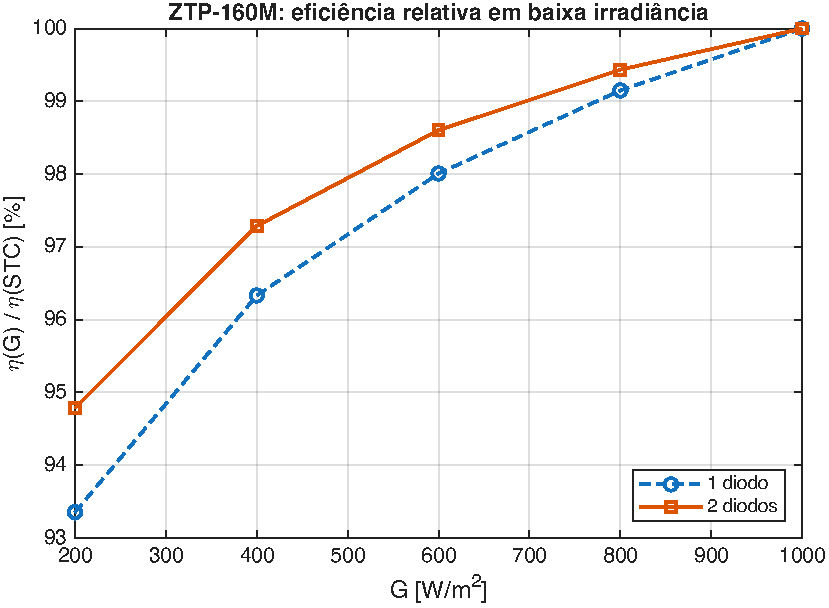
\includegraphics[width=0.48\linewidth]{e1_eficiencia_relativa.pdf}\hfill
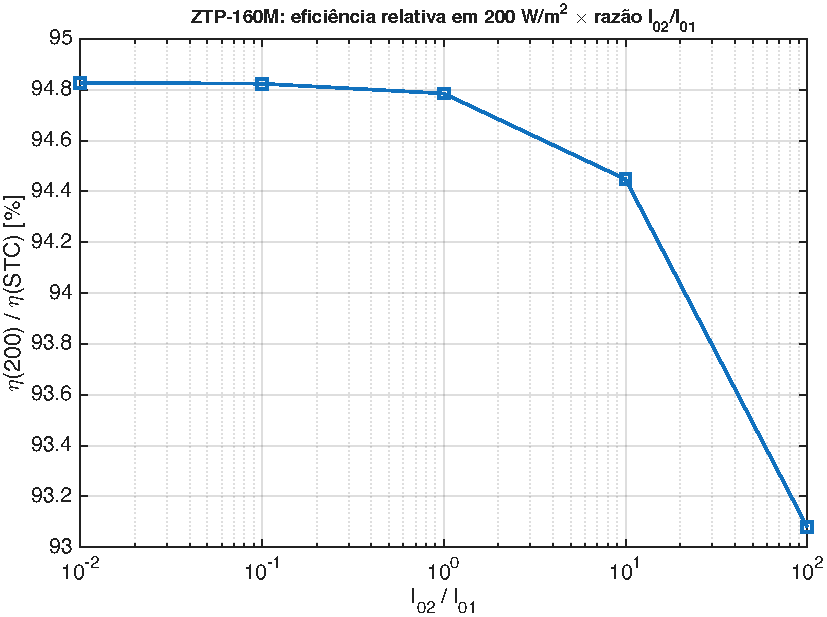
\includegraphics[width=0.48\linewidth]{e1_identificabilidade.pdf}
\caption{E1. Esquerda: efici\^encia relativa $\eta(G)/\eta(\text{STC})$ nos modelos de 1 e 2
diodos. Direita: efici\^encia em 200\,W/m$^2$ em fun\c{c}\~ao de $I_{02}/I_{01}$.}
\label{fig:e1}
\end{figure}

\section{Sombreamento parcial e diodos de bypass}\label{sec:sombra}

Arquivos: \arq{painel/painel_sombreado.m}, \arq{painel/residuo_painel.m},
\arq{cenarios/aplicar_sombras.m}. Aqui o m\'odulo deixa de ser um bloco \'unico e vira tr\^es
subm\'odulos em s\'erie, cada um com a sua irradi\^ancia.

\subsection{A f\'isica}

Em s\'erie, todos os subm\'odulos conduzem a mesma corrente $I$ e as tens\~oes somam. Se um
subm\'odulo recebe pouca luz, n\~ao consegue gerar essa corrente; sem prote\c{c}\~ao seria for\c{c}ado
a tens\~ao negativa e esquentaria (ponto quente). O \textbf{diodo de bypass}, em antiparalelo,
conduz quando a tens\~ao do subm\'odulo cai para cerca de $-0{,}4$\,V: a corrente passa por ele e o
subm\'odulo sombreado deixa de contribuir com tens\~ao. O c\'odigo modela o bypass como um Schottky
($I_{0bp}=1{,}4\times10^{-6}$\,A, queda de $\sim$0,4\,V a 8\,A).

\begin{figure}[htbp]
\centering
\begin{circuitikz}[scale=0.85,transform shape]
  \foreach \y/\i in {0/1,2.8/2,5.6/3} {
    \draw (0,\y) -- (0,\y+0.6) to[battery2,l=$V_\i$] (0,\y+2.2) -- (0,\y+2.8);
    \draw (0,\y+0.6) -- (2.6,\y+0.6) to[D,l_=bypass $\i$] (2.6,\y+2.2) -- (0,\y+2.2);
  }
  \draw (0,8.4) to[short,-o] (0,8.9) node[above]{$+$};
  \draw (0,0) to[short,-o] (0,-0.5) node[below]{$-$};
  \node[font=\scriptsize,gray,anchor=west] at (5.2,4.7) {a mesma corrente $I$ atravessa os tr\^es};
  \node[font=\scriptsize,gray,anchor=west] at (5.2,4.2) {$V_{pv}=V_1+V_2+V_3$};
  \node[font=\scriptsize,gray,anchor=west] at (5.2,3.4) {o bypass fica em reverso};
  \node[font=\scriptsize,gray,anchor=west] at (5.2,2.9) {enquanto o subm\'odulo est\'a iluminado};
\end{circuitikz}
\caption{Tr\^es subm\'odulos em s\'erie, cada um com seu diodo de bypass em antiparalelo. Esquema conceitual.}
\label{fig:bypass}
\end{figure}

\subsection{As equa\c{c}\~oes}

O vetor de inc\'ognitas \'e $z=[I;\,V_{d,1};\dots;V_{d,N}]$, com $V_{d,j}$ a tens\~ao de jun\c{c}\~ao
do subm\'odulo $j$. Dado $V_{d,j}$, tudo no subm\'odulo \'e expl\'icito:
\begin{align}
I_{c,j}&=I_{pv,j}-I_{01}\big(e^{V_{d,j}/(a_1V_t)}-1\big)-I_{02}\big(e^{V_{d,j}/(a_2V_t)}-1\big)-\frac{V_{d,j}}{R_{p,j}}\\
V_j&=V_{d,j}-R_sI_{c,j}\\
I_{bp,j}&=I_{0bp}\big(e^{-V_j/V_{t,bp}}-1\big)
\end{align}
O sistema tem $N+1$ equa\c{c}\~oes:
\begin{align}
R_j&=I_{c,j}+I_{bp,j}-I=0 &&\text{(KCL: c\'elulas + bypass = corrente da fileira)}\\
R_{N+1}&=\textstyle\sum_jV_j-V_{pv}=0 &&\text{(KVL: a tens\~ao do terminal \'e a soma)}
\end{align}

\codigointeiro{painel/residuo_painel.m}{res\'iduo $R(z)$ e jacobiano anal\'itico $J=dR/dz$.}{lst:residuo}

\begin{logica}
\begin{enumerate}
\item \texttt{celula\_params} entrega, para cada subm\'odulo, $R_p$, $I_{pv}$, $I_{01}$, $I_{02}$ (um valor por
 elemento de $G$).
\item \texttt{Ic} \'e a corrente das c\'elulas; \texttt{Vj} a tens\~ao nos terminais do subm\'odulo;
 \texttt{Ibp} a do bypass. Se \texttt{Vj} \'e negativo, \texttt{exp(-Vj/Vt\_bp)} dispara e o bypass
 conduz muito.
\item \texttt{R} empilha as $N$ equa\c{c}\~oes de KCL e a de KVL.
\item \textbf{Jacobiano anal\'itico:} $\partial R_j/\partial I=-1$; $\partial R_j/\partial V_{d,j}=-g-h\,dV_j$
 (com $g=-dI_c/dV_d$, $h=-dI_{bp}/dV_j$, $dV_j=1+R_sg$); a \'ultima linha \'e $dV_j$ (derivada da soma de tens\~oes).
\end{enumerate}
\end{logica}

\subsection{Newton--Raphson com passo limitado}

\codigointeiro{painel/painel_sombreado.m}{corrente do m\'odulo sob sombra por Newton.}{lst:newton}

\begin{logica}
\begin{enumerate}
\item \textbf{Chute inicial.} Sem \emph{warm start}: $I_0=I_{pv,n}\min(G)/G_n$ e $V_d=V_{pv}/N+0{,}5V_t$. Com
 \emph{warm start}, usa-se a solu\c{c}\~ao do ponto anterior.
\item A cada itera\c{c}\~ao calcula-se $R$ e $J$; para se $\|R\|_\infty<10^{-9}$; sen\~ao $\Delta z=-J^{-1}R$.
\item \textbf{Limite de passo:} a corrente muda no m\'aximo 2\,A e cada $V_d$ no m\'aximo $2V_t$ por itera\c{c}\~ao.
 Sem isso, um passo grande de exponencial estoura (overflow).
\item M\'aximo de 60 itera\c{c}\~oes; se n\~ao convergir, avisa com \texttt{warning}.
\item Sa\'idas auxiliares (\texttt{sol.Vj}, \texttt{sol.Ibp}\ldots) servem aos testes de bypass.
\end{enumerate}
\end{logica}

\subsection{O que sai: curvas P-V com v\'arios picos}

O experimento E2 mede os picos de tr\^es cen\'arios do ZTP-160M a 25\,$^\circ$C:

\begin{resultado}
\small\centering
\begin{tabular}{@{}llccc@{}}
\toprule
Cen\'ario & Irradi\^ancia relativa & $V$ [V] & $P$ [W] & Global? \\ \midrule
Sem sombra & [1 1 1] & 19,57 & 160,5 & sim \\
1 subm\'odulo a 40\,\% & [1 1 0,4] & 12,68 & 103,8 & \textbf{sim} \\
1 subm\'odulo a 40\,\% & [1 1 0,4] & 20,69 & 70,2 & n\~ao \\
Degrad\^e 100/60/30\,\% & [1 0,6 0,3] & 5,80 & 47,3 & n\~ao \\
Degrad\^e 100/60/30\,\% & [1 0,6 0,3] & 13,08 & 65,9 & \textbf{sim} \\
Degrad\^e 100/60/30\,\% & [1 0,6 0,3] & 20,49 & 52,2 & n\~ao \\
\bottomrule
\end{tabular}
\end{resultado}

No caso de 1 subm\'odulo a 40\,\%, o pico mais pr\'oximo de $\Voc$ (20,7\,V, 70\,W) \'e local. Um
algoritmo que parta de $\Voc$ e suba a ladeira termina ali e perde 33\,W (32\,\%) em rela\c{c}\~ao ao
pico global de 12,7\,V. No degrad\^e, o global est\'a no meio. Os picos globais sombreados ficam
em 12,7 e 13,1\,V, perto da bateria de 12\,V, e outros ficam abaixo: por isso o conversor precisa
operar como buck \emph{e} como boost (D3).

\begin{figure}[htbp]
\centering
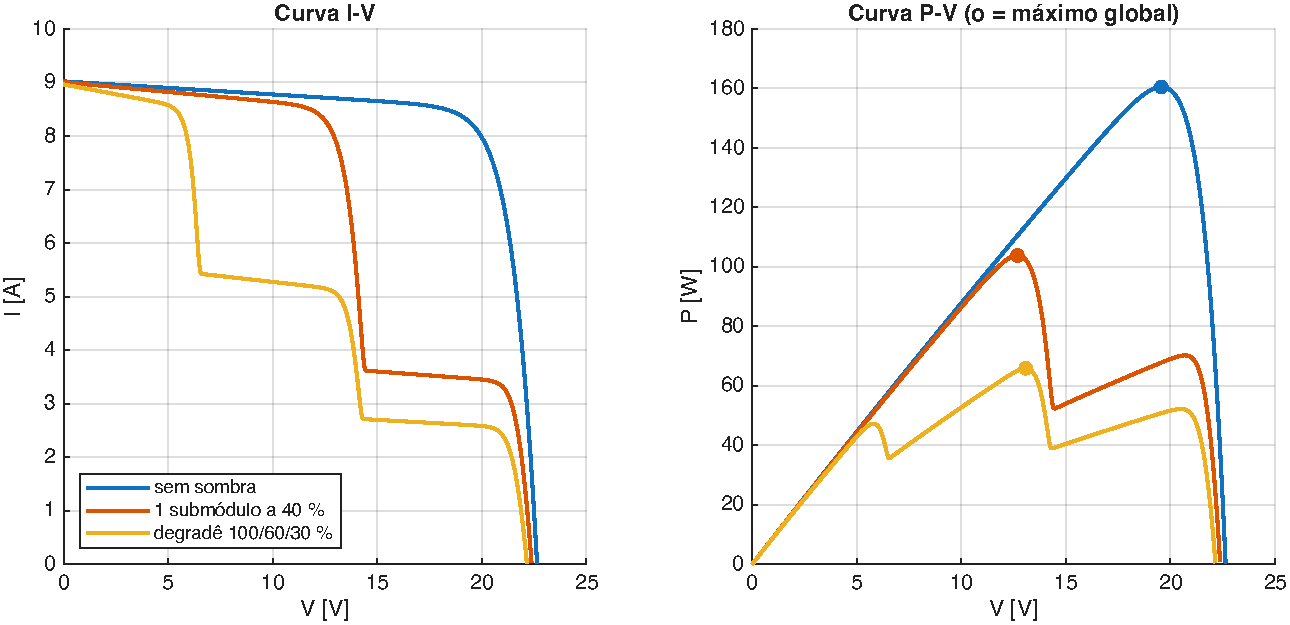
\includegraphics[width=0.92\linewidth]{e2_curvas_sombra.pdf}
\caption{E2. Curvas I-V e P-V do ZTP-160M sob tr\^es padr\~oes de sombra: aparecem de 1 a 3 picos.}
\label{fig:e2}
\end{figure}

\section{Modelo t\'ermico e calibra\c{c}\~ao pelo NMOT}\label{sec:termico}

Arquivos: \arq{termico/termico_dTdt.m}, \arq{parametros_termicos.m}, \arq{calibrar_nmot.m}. A
temperatura do painel muda a curva I-V (Cap\'itulo~\ref{sec:painel}) e portanto muda onde est\'a o
ponto de m\'axima pot\^encia. Ignor\'a-la superestima a energia em cerca de 9\,\% no dia simulado.

\subsection{O balan\c{c}o de energia}

O m\'odulo \'e tratado como um \'unico corpo \`a temperatura $T$ (par\^ametros concentrados). A
energia que entra menos a que sai aquece o m\'odulo:
\begin{equation}\label{eq:termico}
m c_p\frac{dT}{dt}=\underbrace{\alpha AG}_{\text{sol absorvido}}
-\underbrace{P_{el}}_{\text{eletricidade}}
-\underbrace{h_c\,2A\,(T-T_{amb})}_{\text{convec\c{c}\~ao}}
-\underbrace{\varepsilon\sigma A\,(T^4-T_{c\acute eu}^4)}_{\text{radia\c{c}\~ao, frente}}
-\underbrace{\varepsilon\sigma A\,(T^4-T_{amb}^4)}_{\text{radia\c{c}\~ao, verso}}
\end{equation}

\begin{figure}[htbp]
\centering
\begin{tikzpicture}
  \node[bloco,minimum width=4.2cm,minimum height=2.0cm,draw=azul,fill=azul!8] (m) at (0,0)
     {\textbf{M\'odulo a $T$}\\{\scriptsize $m c_p\,dT/dt$ = soma dos fluxos}};
  \node[dest,minimum width=2.6cm] (sol) at (-5.6,2.0) {Sol absorvido\\{\scriptsize $\alpha A G$}};
  \node[aviso,minimum width=2.6cm] (el) at (-5.6,0) {Eletricidade\\{\scriptsize $P_{el}$ (n\~ao vira calor)}};
  \node[bloco,minimum width=2.6cm] (cv) at (5.6,2.0) {Convec\c{c}\~ao\\{\scriptsize $h_c\,2A\,(T-T_{amb})$}};
  \node[bloco,minimum width=2.6cm] (rf) at (5.6,0) {Radia\c{c}\~ao frente\\{\scriptsize para o c\'eu ($T_{c\acute eu}$)}};
  \node[bloco,minimum width=2.6cm] (rv) at (5.6,-2.0) {Radia\c{c}\~ao verso\\{\scriptsize para o solo ($T_{amb}$)}};
  \draw[seta] (sol) -- node[rot,above]{+} (m.north west);
  \draw[seta] (m.west) -- node[rot,above]{$-$} (el);
  \draw[seta] (m.north east) -- node[rot,above]{$-$} (cv);
  \draw[seta] (m.east) -- node[rot,above]{$-$} (rf);
  \draw[seta] (m.south east) -- node[rot,below]{$-$} (rv);
\end{tikzpicture}
\caption{Fluxos de energia do modelo t\'ermico. A radia\c{c}\~ao de onda longa da frente troca com o
c\'eu (frio); a do verso, com o solo (perto de $T_{amb}$).}
\label{fig:termico}
\end{figure}

\begin{center}\small
\begin{tabular}{@{}lll@{}}
\toprule
Termo & Significado f\'isico & Valor \\ \midrule
$\alpha$ & Fra\c{c}\~ao da luz absorvida & 0,9 \\
$P_{el}$ & Energia que sai como eletricidade, n\~ao aquece & vem da simula\c{c}\~ao \\
$h_c$ & Convec\c{c}\~ao de Watmuff: $k_h(2{,}8+3{,}0\,v)$ & $k_h$ calibrado \\
$2A$ & A convec\c{c}\~ao age nas duas faces & $A=0{,}82$\,m$^2$ \\
$\varepsilon$ & Emissividade do vidro & 0,85 \\
$T_{c\acute eu}$ & Temperatura efetiva do c\'eu (Swinbank): $0{,}0552\,T_{amb}^{1{,}5}$ & $\approx277$\,K com $T_{amb}=293$\,K \\
$m c_p$ & Capacidade t\'ermica por \'area: massa $\cdot$ 840\,J/(kg\,K) $/$ \'area & $\approx9{,}1$\,kJ/(m$^2$K) \\
\bottomrule
\end{tabular}
\end{center}

\codigointeiro{termico/termico_dTdt.m}{o balan\c{c}o de energia como fun\c{c}\~ao $dT/dt$.}{lst:termico}

\begin{logica}
\begin{enumerate}
\item \texttt{hc = kh*(2.8 + 3.0*vw)}: coeficiente de convec\c{c}\~ao; \texttt{At = 2*A} porque o ar toca as duas faces.
\item \texttt{Tceu = 0.0552*Tamb\^{}1.5}: temperatura efetiva do c\'eu; \'e a que a face da frente ``enxerga''.
\item \texttt{Q\_sol}, \texttt{Q\_conv}, \texttt{Q\_rad\_frente}, \texttt{Q\_rad\_tras}: cada fluxo em watts.
\item \texttt{dTdt = (Q\_sol - Pel - Q\_conv - Q\_rad)/(mcp\_area*A)}: o saldo dividido pela capacidade t\'ermica total em J/K.
\end{enumerate}
\end{logica}

Duas escolhas merecem explica\c{c}\~ao (D11):
\begin{itemize}
\item \textbf{Watmuff, n\~ao McAdams.} O coeficiente de McAdams ($5{,}7+3{,}8v$) j\'a inclui a
 radia\c{c}\~ao. Como o c\'odigo calcula a radia\c{c}\~ao \`a parte, usar McAdams contaria a radia\c{c}\~ao duas vezes.
\item \textbf{Frente v\^e o c\'eu, verso v\^e o solo.} Com tudo irradiando para o c\'eu, a calibra\c{c}\~ao
 pelo NMOT exigia $k_h=0{,}33$, valor irreal.
\end{itemize}
A capacidade t\'ermica vem da massa do datasheet (8,9\,kg): o vidro \'e 70 a 75\,\% da massa e tem
$c_p\approx840$\,J/(kg\,K); alum\'inio ($\sim$900) e pol\'imeros (1200 a 1500) s\~ao fra\c{c}\~oes menores.

\subsection{Calibra\c{c}\~ao pelo NMOT}

O \'unico par\^ametro livre \'e $k_h$. Ele \'e ajustado para reproduzir o \textbf{NMOT}, publicado no
datasheet como 45\,$^\circ$C, nas condi\c{c}\~oes $G=800$\,W/m$^2$, $T_{amb}=20\,^\circ$C, vento de
1\,m/s, m\'odulo no MPP.

\codigointeiro{termico/calibrar_nmot.m}{busca do $k_h$ que zera $dT/dt$ em 45\,$^\circ$C.}{lst:nmot}

\begin{logica}
\begin{enumerate}
\item Pot\^encia el\'etrica no NMOT estimada pelo datasheet:
 $P_{el}=P_{max}\cdot0{,}8\cdot(1+\gamma_P(45-25))=160\cdot0{,}8\cdot0{,}92\approx117{,}8$\,W.
\item Em regime permanente $dT/dt=0$. \texttt{fzero} procura em $[0{,}1;\,10]$ o $k_h$ que zera
 \texttt{balanco\_com\_kh} em $T=45\,^\circ$C.
\item Resultado: $\boldsymbol{k_h=0{,}79}$.
\end{enumerate}
\end{logica}

\begin{resultado}
\textbf{Conferindo \`a m\~ao.} Com $k_h=0{,}79$ e vento de 1\,m/s, $h_c\approx4{,}6$\,W/(m$^2$K). Em
$T=45\,^\circ$C: sol absorvido $\approx590$\,W; el\'etrico $\approx118$\,W; convec\c{c}\~ao $\approx188$\,W;
radia\c{c}\~ao frente $\approx172$\,W; radia\c{c}\~ao verso $\approx113$\,W. Saldo:
$590-118-188-172-113\approx0$.

\textbf{Constante de tempo.} Capacidade total $9{,}1\text{ kJ/(m}^2\text{K)}\times0{,}82\text{ m}^2\approx7{,}5$\,kJ/K.
A perda cresce $\approx17{,}7$\,W por kelvin. Logo $\tau\approx7{,}5/17{,}7\approx7$\,min, na faixa t\'ipica de 5 a 7\,min.
\end{resultado}

\begin{atencao}[: cuidado num\'erico]
Com vento de 10\,m/s a menor constante de tempo cai para $\sim$2,3\,min. No Euler expl\'icito o passo
precisa ser menor que $2\tau$ (na pr\'atica bem menor que 1\,min). A simula\c{c}\~ao quase-est\'atica
usa passo $\Ta\approx31$\,ms (est\'avel de sobra); a din\^amica usa \texttt{ode15s}. O vento do PVGIS
\'e a 10\,m de altura e \'e convertido para o vento junto ao m\'odulo no c\'odigo do cen\'ario.
\end{atencao}

\section{Conversor buck-boost}\label{sec:conversor}

Arquivos: \arq{conversor/parametros_conversor.m}, \arq{conversor_ideal.m}, \arq{conversor_medio_rhs.m},
\arq{equilibrio_conversor.m}, \arq{verifica_ccm.m}, \arq{sim_chaveado.m}, \arq{sim_medio_aberta.m}.
O conversor \'e quem imp\~oe ao painel a tens\~ao de opera\c{c}\~ao. Sem ele n\~ao h\'a como o MPPT
``escolher'' o ponto da curva.

\subsection{Como funciona o buck-boost inversor}

O conversor tem uma chave (MOSFET), um indutor $L$, um diodo Schottky e um capacitor $C$ na
entrada, em paralelo com o painel. Em cada per\'iodo $T_s=1/f_s$:

\begin{itemize}
\item \textbf{Chave ligada} (fra\c{c}\~ao $d$ do per\'iodo, a \emph{raz\~ao c\'iclica}): o indutor fica
 ligado ao painel e \emph{carrega}; a corrente $i_L$ sobe.
\item \textbf{Chave desligada} (fra\c{c}\~ao $1-d$): o indutor \'e desligado do painel e
 \emph{descarrega} na bateria pelo diodo; $i_L$ cai.
\end{itemize}

\begin{figure}[htbp]
\centering
\begin{circuitikz}[scale=0.9,transform shape]
  \draw (0,0) to[isource,l_=Painel] (0,3) -- (1.8,3);
  \draw (1.8,3) to[C,l=$C$] (1.8,0);
  \draw (1.8,3) to[cspst,l=$S$] (4.3,3);
  \draw (4.3,3) to[L,l=$L$] (4.3,0);
  \draw (4.3,3) -- (5,3) to[D,l_=$D$] (7,3) -- (7,2.4);
  \draw (7,2.4) to[battery2,l=$V_{bat}$] (7,0.6) -- (7,0);
  \draw (0,0) -- (7,0);
  \node[font=\scriptsize] at (7.45,0.45) {$+$};
  \node[font=\scriptsize] at (7.45,2.55) {$-$};
  \node[font=\scriptsize,gray,anchor=west] at (2.2,-0.7) {Polaridade invertida: a bateria \'e carregada pela corrente do diodo.};
\end{circuitikz}
\caption{Conversor buck-boost inversor, entre o painel (com o capacitor de entrada $C$) e a bateria.}
\label{fig:circuito_conv}
\end{figure}

\begin{figure}[htbp]
\centering
\begin{tikzpicture}
  \node[ctrl,minimum width=6.4cm,minimum height=2.1cm,align=left] (on) at (0,0)
    {\textbf{Chave ligada, fra\c{c}\~ao $d$}\\[2pt]{\scriptsize $L\,\dfrac{di_L}{dt}=\vpv-i_L(r_L+R_{on})$}\\[4pt]{\scriptsize $C\,\dfrac{d\vpv}{dt}=\ipv-i_L$}};
  \node[dest,minimum width=6.4cm,minimum height=2.1cm,align=left] (off) at (7.4,0)
    {\textbf{Chave desligada, fra\c{c}\~ao $1-d$}\\[2pt]{\scriptsize $L\,\dfrac{di_L}{dt}=-(V_{bat}+V_F)-i_L(r_L+R_D)$}\\[4pt]{\scriptsize $C\,\dfrac{d\vpv}{dt}=\ipv$}};
  \draw[seta,bend left=18] (on.north east) to node[rot,above]{$d\,T_s$} (off.north west);
  \draw[seta,bend left=18] (off.south west) to node[rot,below]{$(1-d)\,T_s$} (on.south east);
\end{tikzpicture}
\caption{As duas topologias que se alternam a cada per\'iodo de chaveamento.}
\label{fig:duas_topologias}
\end{figure}

No regime permanente a tens\~ao m\'edia no indutor \'e zero (o fluxo n\~ao pode crescer sem limite).
Sem perdas isso d\'a $d\,\vpv=(1-d)\,V_{bat}$, ou
\begin{equation}\label{eq:d_ideal}
d=\frac{V_{bat}}{V_{bat}+\vpv},\qquad i_L=\frac{\ipv}{d}.
\end{equation}
A raz\~ao c\'iclica \'e a ``alavanca'' do MPPT: mudar $d$ muda $\vpv$. Com $V_{bat}=12$\,V e
$\vpv=19{,}57$\,V (MPP de STC), $d=0{,}38<0{,}5$: o conversor trabalha como buck. Se o pico global
cai para 7\,V, $d=0{,}63$ e trabalha como boost.

\subsection{Dimensionamento}

\codigointeiro{conversor/parametros_conversor.m}{$L$ e $C$ pelo ripple no MPP de STC, perdas t\'ipicas.}{lst:paramconv}

\begin{logica}
\begin{enumerate}
\item Ponto de projeto: MPP de STC (\texttt{curva\_pv} com $G=1000$ em todos os subm\'odulos).
\item $D=V_{bat}/(V_{bat}+V_{mp})\approx0{,}380$ e $I_L=I_{mp}/D\approx21{,}6$\,A (eq.~\ref{eq:d_ideal}).
\item \textbf{Indutor}: com a chave ligada, $\Delta i=\vpv D T_s/L$. Impondo ripple de 30\,\% de $I_L$:
 $L=V_{mp}D/(0{,}30\,I_Lf_s)\approx57\,\mu$H.
\item \textbf{Capacitor}: com a chave ligada o indutor puxa $i_L$ do capacitor; a carga trocada por ciclo \'e
 $I_LD(1-D)T_s$. Com ripple de tens\~ao de 1\,\%: $C=I_LD(1-D)/(0{,}01\,V_{mp}f_s)\approx1{,}3$\,mF.
\item Perdas de cat\'alogo: $r_L=20$\,m$\Omega$, $R_{on}=18$\,m$\Omega$, $V_F=0{,}45$\,V, $R_D=10$\,m$\Omega$,
 $t_r+t_f=100$\,ns; limites $d\in[0{,}02;\,0{,}95]$; atraso do PWM $1{,}5T_s=75\,\mu$s.
\end{enumerate}
\end{logica}

O ripple real fica em $\sim$34 a 35\,\%, n\~ao 30\,\%, porque o $d$ real (com perdas) \'e maior que o ideal usado
no projeto. A MOSFET \'e de classe 60\,V porque a chave v\^e $\vpv+V_{bat}\approx37$\,V. As perdas s\~ao t\'ipicas de
cat\'alogo, e o E7 mede o efeito delas (com e sem perdas), ent\~ao a conclus\~ao n\~ao depende dos valores exatos.

\subsection{Tr\^es modelos do mesmo conversor}

\begin{center}\small
\begin{tabularx}{\textwidth}{@{}lXX@{}}
\toprule
Modelo & O que faz & Quando usar \\ \midrule
\textbf{Ideal} (\arq{conversor_ideal}) & Zera todas as perdas & Compara\c{c}\~ao: ``quanto as perdas custam?'' \\
\textbf{M\'edio com perdas} (\arq{conversor_medio_rhs}) & M\'edia ponderada pelo tempo das duas topologias; sem ripple & Simula\c{c}\~oes longas (dia inteiro) \\
\textbf{Chaveado} (\arq{sim_chaveado}) & Alterna as topologias de fato, 200 passos por per\'iodo & S\'o para validar o m\'edio, em janelas de ms \\
\bottomrule
\end{tabularx}
\end{center}

\subsubsection{Modelo m\'edio}

\begin{equation}\label{eq:medio}
C\frac{d\vpv}{dt}=\ipv-d\,i_L,\qquad
L\frac{di_L}{dt}=d\,\vpv-(1-d)(V_{bat}+V_F)-i_L\big(r_L+d\,R_{on}+(1-d)R_D\big)
\end{equation}

\codigointeiro{conversor/conversor_medio_rhs.m}{lado direito do modelo m\'edio.}{lst:medio}

\begin{logica}
Cada termo da eq.~\eqref{eq:medio} \'e a m\'edia ponderada pelo tempo das duas topologias da
Figura~\ref{fig:duas_topologias}: o que ocorre com a chave ligada multiplica-se por \texttt{d}; o que ocorre
com ela desligada, por \texttt{(1-d)}. O capacitor s\'o \'e descarregado pelo indutor durante a fra\c{c}\~ao
\texttt{d}.
\end{logica}

\subsubsection{Modelo chaveado}

\codigo{conversor/sim_chaveado.m}{44}{85}{o la\c{c}o de Euler com 200 passos por per\'iodo.}{lst:chaveado}

\begin{logica}
\begin{enumerate}
\item A cada passo guarda-se o estado \emph{antes} de avan\c{c}ar; \texttt{j} \'e o \'indice do passo dentro do per\'iodo.
\item \textbf{PWM real:} $d$ \'e amostrado no in\'icio de cada per\'iodo (\texttt{j == 0}) e fica fixo at\'e o pr\'oximo.
\item \texttt{f} \'e a fra\c{c}\~ao do passo com a chave ligada: 1 antes de $d\cdot200$, 0 depois, e fracion\'ario no passo da
 comuta\c{c}\~ao. Sem isso o $d$ efetivo erraria em at\'e $1/200$.
\item O painel \'e resolvido por Newton (com \emph{warm start}) na tens\~ao atual do capacitor.
\item As derivadas das duas topologias s\~ao combinadas por \texttt{f} e o estado avan\c{c}a por Euler.
\item O diodo bloqueia corrente reversa: \texttt{iL = max(..., 0)}. Quando $i_L$ chega a zero, entra-se em DCM.
\end{enumerate}
A condi\c{c}\~ao inicial parte do instante em que a chave liga ($i_L$ no vale, $\vpv$ no pico): partir da m\'edia
deslocaria o resultado em meio ripple ($\sim$17\,\% em STC) e excitaria uma oscila\c{c}\~ao LC que n\~ao existe no modelo m\'edio.
\end{logica}

\subsection{O equil\'ibrio com perdas}

Dado $(\vpv,\ipv)$, \arq{equilibrio_conversor} acha $d$ e a efici\^encia. Em regime, $d\vpv/dt=0$ d\'a
$i_L=\ipv/d$. Substituindo em $di_L/dt=0$ e multiplicando por $d$, chega-se a uma equa\c{c}\~ao do 2.\textordmasculine\ grau:
\begin{equation}\label{eq:quadratica}
(\vpv+V_t)\,d^2-\big(V_t+\ipv(R_{on}-R_D)\big)\,d-\ipv(r_L+R_D)=0,\qquad V_t=V_{bat}+V_F .
\end{equation}
O coeficiente de $d^2$ \'e positivo e o termo constante \'e negativo: o produto das ra\'izes \'e negativo e h\'a
\textbf{exatamente uma raiz positiva}. N\~ao precisa de \texttt{fzero}.

\codigointeiro{conversor/equilibrio_conversor.m}{raiz da quadr\'atica, perdas e efici\^encia.}{lst:equilibrio}

\begin{logica}
\begin{enumerate}
\item Se $\ipv\le0$ (noite): sem transfer\^encia, devolve tudo zerado e \texttt{viavel = false}.
\item \texttt{a}, \texttt{b}, \texttt{c} s\~ao os coeficientes de (\ref{eq:quadratica}); \texttt{d} \'e a raiz positiva.
\item Se $d$ sai de $[D_{min},D_{max}]$ o controlador n\~ao alcan\c{c}a o ponto: tamb\'em sem transfer\^encia.
\item \textbf{Perda de condu\c{c}\~ao:} $P_{cond}=i_L^2(r_L+dR_{on}+(1-d)R_D)+(1-d)i_LV_F$.
\item \textbf{Perda de chaveamento:} $P_{sw}=\tfrac12(\vpv+V_{bat})\,i_L\,(t_r+t_f)\,f_s$ (sobreposi\c{c}\~ao tens\~ao $\times$ corrente).
\item \textbf{Pot\^encia na bateria:} $P_{out}=(1-d)\,i_LV_{bat}-P_{sw}$; $\eta=P_{out}/(\vpv\ipv)$.
\end{enumerate}
$P_{sw}$ entra s\'o no balan\c{c}o de pot\^encia, n\~ao na EDO m\'edia ($<1$\,\% em STC).
\end{logica}

\subsection{CCM e DCM}

\codigointeiro{conversor/verifica_ccm.m}{teste de condu\c{c}\~ao cont\'inua.}{lst:ccm}

O ripple pico a pico \'e $\vpv\,d/(L f_s)$ e a condu\c{c}\~ao \'e cont\'inua (\textbf{CCM}) se $i_L>\text{ripple}/2$.
Em baixa luz (50\,W/m$^2$) a corrente m\'edia ($\sim$1\,A) \'e menor que meio ripple ($\sim$3\,A): o conversor entra em
\textbf{condu\c{c}\~ao descont\'inua (DCM)}. Ali o modelo m\'edio de CCM deixa de valer e a efici\^encia calculada fica
\emph{otimista}, pois as perdas de condu\c{c}\~ao dependem da corrente RMS, bem maior que a m\'edia.

\subsection{Valida\c{c}\~ao chaveado $\times$ m\'edio (E3)}

O experimento aplica um degrau de $+0{,}02$ em $d$, em $t=2$\,ms, partindo do MPP, e compara o modelo m\'edio com a m\'edia
m\'ovel de um per\'iodo do chaveado.

\begin{itemize}
\item \textbf{Em STC (CCM):} o m\'edio segue o chaveado. O teste de regress\~ao exige desvio m\'aximo $<0{,}5$\,\% na tens\~ao e
 $<1{,}5$\,\% na corrente, e ripple de $i_L$ dentro de 15\,\% do valor te\'orico.
\item \textbf{Em 50\,W/m$^2$ (DCM):} as curvas se separam, e isso \'e o resultado esperado. Em DCM a energia puxada por
 ciclo \'e fixada por $(\vpv dT_s)^2/(2L)$, muito maior que a pot\^encia do painel nessa luz; o m\'edio chega a dar
 $i_L<0$, imposs\'ivel fisicamente. O experimento mostra o \emph{limite de validade} do modelo m\'edio.
\end{itemize}

\begin{figure}[htbp]
\centering
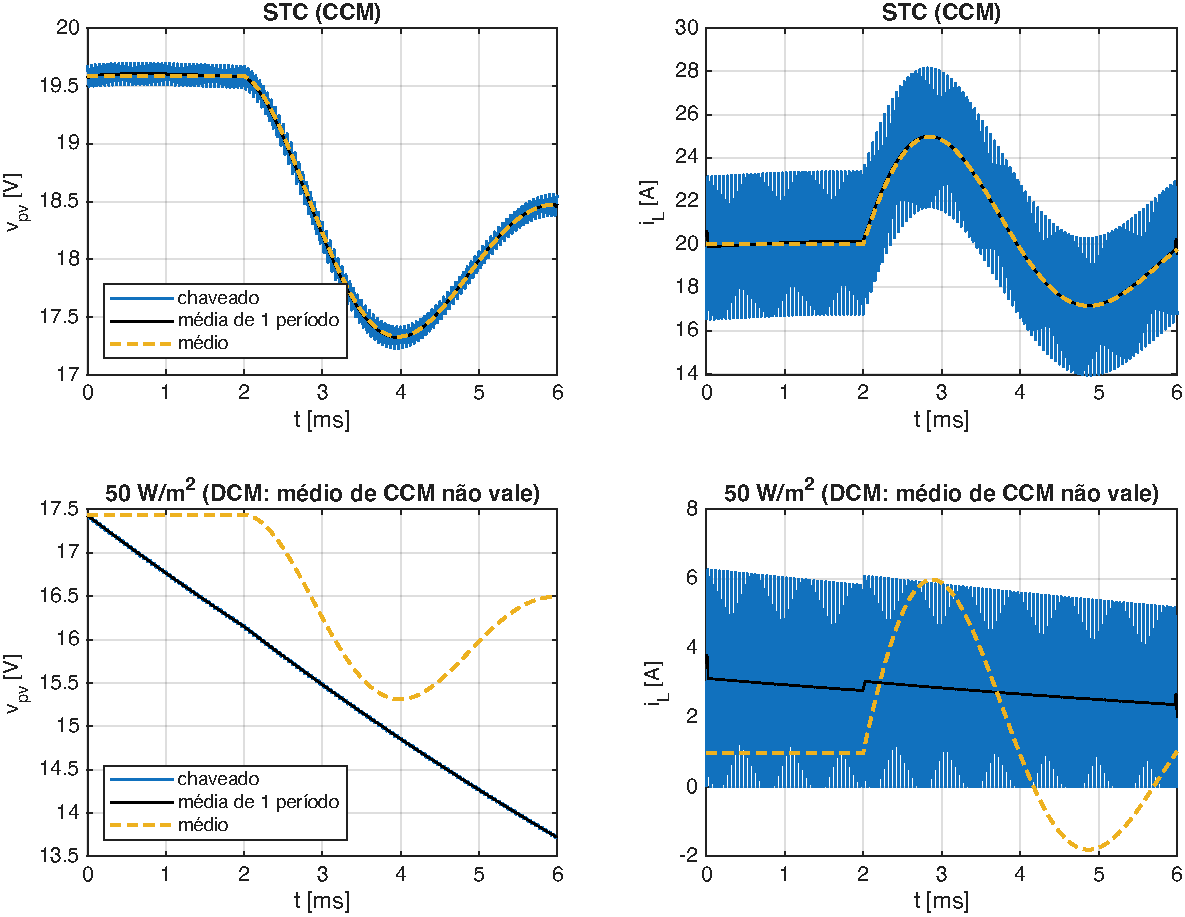
\includegraphics[width=0.9\linewidth]{e3_chaveado_medio.pdf}
\caption{E3. Modelo chaveado (com ripple), m\'edia m\'ovel de um per\'iodo e modelo m\'edio. Em cima, STC (CCM); embaixo,
50\,W/m$^2$ (DCM).}
\label{fig:e3}
\end{figure}

\subsection{Malha aberta com DAE (\texttt{sim\_medio\_aberta})}

Integra o modelo m\'edio mais o painel como DAE (equa\c{c}\~oes diferenciais e alg\'ebricas) com \texttt{ode15s} e matriz de
massa $M=\mathrm{diag}(1,1,0,\dots,0)$: as duas primeiras linhas s\~ao EDOs ($\vpv$ e $i_L$) e as demais s\~ao as
restri\c{c}\~oes alg\'ebricas do painel. O jacobiano anal\'itico \'e obrigat\'orio, pois com diferen\c{c}as finitas a
exponencial do bypass faz o \texttt{ode15s} falhar. Ela s\'o \'e usada no E3; a malha fechada usa a EDO reduzida
(Cap\'itulo~\ref{sec:sim}), porque a DAE falhou em 9 de 36 casos quando o MPPT dava degraus grandes.

\section{Controle: lineariza\c{c}\~ao, resposta em frequ\^encia e projeto do PI}\label{sec:controle}

Arquivos: \arq{controle/linearizar_planta.m}, \arq{gvd_analitico.m}, \arq{resposta_freq.m},
\arq{margens.m}, \arq{projeto_pi.m}, \arq{resposta_degrau_mf.m}, \arq{lei_pi.m}. O MPPT n\~ao mexe na
raz\~ao c\'iclica $d$ diretamente: ele escolhe uma tens\~ao de refer\^encia $\Vref$, e um \textbf{PI de
tens\~ao} ajusta $d$ para que $\vpv$ siga $\Vref$. Este cap\'itulo mostra como esse PI foi projetado.

\subsection{A estrutura em dois la\c{c}os}

\begin{itemize}
\item \textbf{La\c{c}o interno (r\'apido):} PI que mede $\vpv$ e ajusta $d$ para seguir $\Vref$; escala de ms.
\item \textbf{La\c{c}o externo (lento):} MPPT que, a cada $\Ta$, escolhe um novo $\Vref$; escala de dezenas de ms.
\end{itemize}

\begin{figure}[htbp]
\centering
\begin{tikzpicture}
  \node[bloco,minimum width=1.6cm,minimum height=1.0cm] (mp) at (0,0) {MPPT};
  \node[circle,draw=cinza,thick,inner sep=1pt] (som) at (2.6,0) {$\Sigma$};
  \node[ctrl,minimum width=2.4cm] (pi) at (5.2,0) {PI\\{\scriptsize $K_p(1+\tfrac{1}{sT_i})$}};
  \node[bloco,minimum width=2.0cm] (atr) at (8.0,0) {Atraso PWM\\{\scriptsize $e^{-1{,}5sT_s}$}};
  \node[bloco,minimum width=2.4cm] (pl) at (11.0,0) {Planta\\{\scriptsize $-G_{vd}(s)$}};
  \draw[seta] (mp) -- node[rot,above]{$\Vref$} (som);
  \draw[seta] (som) -- node[rot,above]{$e$} (pi);
  \draw[seta] (pi) -- node[rot,above]{$d$} (atr);
  \draw[seta] (atr) -- (pl);
  \draw[seta] (pl.east) -- ++(0.7,0) node[rot,above right]{$\vpv$} -- ++(0,-1.5) -| node[rot,below,pos=0.2]{realimenta\c{c}\~ao de $\vpv$} (som.south);
  \draw[seta] ([xshift=0.7cm]pl.east) |- ($(mp.south)+(0,-2.2)$) -- (mp.south);
  \node[rot,anchor=north] at (3,-2.2) {mede $V,I$ a cada $\Ta$};
\end{tikzpicture}
\caption{Malha de tens\~ao do conversor. O ganho de malha \'e $L(s)=C(s)\,[-G_{vd}(s)]\,e^{-1{,}5sT_s}$; o sinal
negativo da planta \'e absorvido na defini\c{c}\~ao do erro.}
\label{fig:malha}
\end{figure}

O la\c{c}o externo s\'o funciona se o interno j\'a tiver acomodado quando o MPPT medir a pot\^encia: esse \'e o crit\'erio que
fixa $\Ta$ (Se\c{c}\~ao~\ref{sec:femia}).

\subsection{Lineariza\c{c}\~ao de pequenos sinais}

O modelo m\'edio \'e n\~ao linear (h\'a o produto $d\,i_L$ e a curva I-V do painel). Para projetar um controlador cl\'assico,
ele \'e linearizado em torno de um equil\'ibrio $(x_0,d_0)$, onde $f(x_0,d_0)=0$. Escreve-se $x=x_0+\tilde x$ e $d=d_0+\tilde d$
com $\tilde x$ e $\tilde d$ pequenos; a s\'erie de Taylor de 1.\textordmasculine\ ordem d\'a
\begin{equation}
\dot{\tilde x}=A\tilde x+B\tilde d,\qquad A=\frac{\partial f}{\partial x}\Big|_{(x_0,d_0)},\quad
B=\frac{\partial f}{\partial d}\Big|_{(x_0,d_0)},\quad \tilde v_{pv}=C\tilde x .
\end{equation}

\codigo{controle/linearizar_planta.m}{34}{80}{equil\'ibrio, matrizes $A$ e $B$ por diferen\c{c}as centrais e $r_{pv}$.}{lst:linear}

\begin{logica}
\begin{enumerate}
\item \textbf{Equil\'ibrio:} resolve o painel em \texttt{op.vpv} e acha $(d_0,i_{L0})$ com \arq{equilibrio_conversor}. Se o ponto for
 invi\'avel, d\'a erro dizendo se foi $\vpv>V_{oc}$ ou $d$ fora de $[D_{min},D_{max}]$.
\item \textbf{Matriz $A$:} perturba cada estado ($h=10^{-5}\max(1,|x_j|)$) e deriva por $(f(x_0+h)-f(x_0-h))/(2h)$, com erro $O(h^2)$.
 Assim a mesma fun\c{c}\~ao serve com ou sem perdas e para qualquer padr\~ao de sombra, sem derivar o painel \`a m\~ao.
\item \textbf{Vetor $B$:} idem, perturbando $d$ ($h=10^{-6}$).
\item \textbf{Resist\^encia din\^amica:} $r_{pv}=-1/(dI/dV)$. No MPP, $dP/dV=I+V\,dI/dV=0$ e $r_{pv}=V_{mp}/I_{mp}$: a din\^amica
 iguala a est\'atica; esse \'e o princ\'ipio do m\'etodo InC.
\item \textbf{CCM?} O modelo linear s\'o vale em condu\c{c}\~ao cont\'inua (\texttt{sys.ccm}).
\end{enumerate}
\end{logica}

\subsection{A planta $G_{vd}$ em forma fechada}

Sem perdas, com o painel virando um resistor $r_{pv}$, as equa\c{c}\~oes de pequenos sinais s\~ao
\begin{equation}
C\dot{\tilde v}=-\frac{\tilde v}{r_{pv}}-D\,\tilde i_L-I_L\,\tilde d,\qquad
L\dot{\tilde i}_L=D\,\tilde v+(V+V_{bat})\,\tilde d .
\end{equation}
Eliminando $\tilde i_L$ na transformada de Laplace:
\begin{equation}\label{eq:gvd}
G_{vd}(s)=\frac{\tilde v_{pv}}{\tilde d}=-\frac{L I_L\,s+D\,(V+V_{bat})}{L C\,s^2+(L/r_{pv})\,s+D^2}
\end{equation}

\codigointeiro{controle/gvd_analitico.m}{$G_{vd}(j\omega)$ sem perdas, para conferir a planta num\'erica.}{lst:gvd}

Tr\^es pontos de leitura:
\begin{itemize}
\item \textbf{Sinal negativo:} mais $d$ = chave mais tempo ligada; o indutor puxa mais corrente do capacitor e $\vpv$ cai.
\item \textbf{Polos:} $\omega_0=D/\sqrt{LC}$ e $\zeta=\sqrt{L/C}/(2D\,r_{pv})$. Com os valores do projeto isso d\'a a
 resson\^ancia LC em $\sim$240\,Hz, pouco amortecida ($\zeta$ de 0,16 a 0,3).
\item \textbf{Amortecimento:} o \'unico ``resistor'' do caso sem perdas \'e o pr\'oprio painel.
\end{itemize}

\codigointeiro{controle/resposta_freq.m}{$H(j\omega)=C(j\omega I-A)^{-1}B+D$, no lugar de \texttt{bode}/\texttt{freqresp}.}{lst:rfreq}

\subsection{Margens de estabilidade sem toolbox}

\texttt{margens(w,L)} substitui \texttt{margin()}. Duas defini\c{c}\~oes:
\begin{itemize}
\item \textbf{Margem de fase (MF):} na frequ\^encia $\omega_c$ onde $|L|=1$, quanto falta para a fase chegar a $-180^\circ$:
 $\mathrm{MF}=180^\circ+\angle L(j\omega_c)$. Se a fase chegasse a $-180^\circ$ com $|L|=1$, $L=-1$ e $1+L=0$: polo de malha
 fechada sobre o eixo imagin\'ario (oscila\c{c}\~ao sustentada). O usual \'e MF $\ge45^\circ$.
\item \textbf{Margem de ganho (MG):} na frequ\^encia onde a fase vale $-180^\circ$, quanto o ganho poderia crescer at\'e
 $|L|=1$: $\mathrm{MG}=-20\log_{10}|L(j\omega_{180})|$. MG $\ge6$\,dB significa que o ganho da planta pode dobrar sem instabilizar.
\end{itemize}

\codigointeiro{controle/margens.m}{margens de fase e ganho a partir de $L(j\omega)$ amostrado.}{lst:margens}

\begin{logica}
\begin{enumerate}
\item \texttt{fase = unwrap(angle(L))*180/pi}: fase cont\'inua, sem saltos de $360^\circ$.
\item \textbf{Cruzamentos de ganho:} varre as amostras e detecta onde $|L|$ passa de $\ge1$ para $<1$ (ou volta). Interpola em
 $\log|L|$, pois no Bode o m\'odulo varia como pot\^encia de $\omega$.
\item \textbf{Cruzamentos de fase:} detecta onde $\text{fase}+180^\circ$ muda de sinal (descartando o salto artificial de $\pm180^\circ$).
\item O c\'odigo olha \textbf{todos} os cruzamentos, n\~ao s\'o o primeiro, e fica com a pior margem: a resson\^ancia LC pode
 fazer $|L|$ voltar a passar de 1 depois do primeiro cruzamento.
\end{enumerate}
\end{logica}

\subsection{O projeto do PI (D12 e D13)}

O controlador \'e $C(s)=K_p(1+1/(sT_i))$, aplicado como $d=K_p(e+\xi/T_i)$ com $e=\vpv-\Vref$ e $\dot\xi=e$.

\begin{atencao}[: por que a regra cl\'assica falha]
A regra usual p\~oe o zero do PI uma d\'ecada abaixo do cruzamento ($\omega_z=\omega_c/5$, $r=0{,}2$). Aqui a planta \'e plana
(40 a 85\,V por unidade de $d$) at\'e a resson\^ancia LC. Com o zero abaixo de $\omega_c$, acima dele o PI vira praticamente s\'o o
ganho $K_p$, e $|L|$ fica perto de 1 desde $\omega_c$ at\'e a resson\^ancia: o pico cruza 0\,dB de novo com fase
$\approx-150^\circ$, e a MF cai para 25 a $40^\circ$. Subir $f_c$ acima da resson\^ancia tamb\'em n\~ao adianta: ali a fase da planta j\'a
est\'a perto de $-180^\circ$.
\end{atencao}

\textbf{O que funciona:} zero \emph{acima} do cruzamento ($r>1$). Abaixo do zero o PI age como integrador puro, $|L|$ cai
20\,dB/d\'ecada, o cruzamento fica bem abaixo da resson\^ancia e $|L|\ll1$ no pico LC. A fase em $\omega_c$ \'e $\approx-90^\circ$, ent\~ao a
MF \'e alta.

\codigo{controle/projeto_pi.m}{114}{170}{varredura de $f_c$ e $r$, escolha do maior $f_c$ que passa e c\'alculo de $\Ta$.}{lst:projpi}

\begin{logica}
\begin{enumerate}
\item Antes deste trecho, o c\'odigo monta os casos de robustez (pr\'oxima subse\c{c}\~ao) e lineariza cada um uma s\'o vez: a planta
 n\~ao depende do PI.
\item Para cada $f_c$ (80 valores, de 5\,Hz a $f_s/10$, espa\c{c}ados em log) e cada $r\in\{0{,}2;0{,}5;1;2;5\}$:
 \texttt{Ti = 1/(r*wc)} e \texttt{Kp} tal que $|L(j\omega_c)|=1$ no ponto nominal.
\item Calcula MF e MG em todos os casos. Se alguma ficar abaixo de $45^\circ$ ou 6\,dB, descarta o par.
\item Para os que passam, simula o degrau de $\Vref$ em cada caso (\texttt{resposta\_degrau\_mf}) e calcula $t_s$ (faixa de 2\,\%).
 Exige $t_{s,max}<50$\,ms, s\'o para rejeitar malhas absurdamente lentas.
\item Entre os aprovados, fica o de \textbf{maior $f_c$} (empate: maior MF): banda maior = malha mais r\'apida = passos de MPPT mais curtos.
\item No fim, $\Ta=1{,}5\,t_{s,max}$ arredondado para cima em ms.
\end{enumerate}
\end{logica}

\subsection{Robustez}

Indutores e capacitores eletrol\'iticos t\^em toler\^ancia t\'ipica de $\pm20$\,\%. Por isso cada ponto de opera\c{c}\~ao \'e
verificado com $L$ e $C$ nominais e nos cantos $[f_L\ f_C]=[1{,}2\ 1],[1\ 1{,}2],[1{,}2\ 1{,}2],[0{,}8\ 0{,}8]$. S\~ao 12 pontos de
opera\c{c}\~ao:
\begin{itemize}
\item 1000, 600 e 200\,W/m$^2$ uniformes, cada um no MPP e em $0{,}8V_{mp}$ e $1{,}1V_{mp}$ (o MPPT passeia em torno do MPP e o ganho muda com $r_{pv}$);
\item os dois picos da curva com um subm\'odulo a 400\,W/m$^2$;
\item o m\'odulo quente (60\,$^\circ$C, 1000\,W/m$^2$) no seu MPP.
\end{itemize}
S\~ao $12\times5=60$ casos. Em 4 deles, em 200\,W/m$^2$, o conversor cai em DCM e eles s\~ao exclu\'idos (o modelo linear de CCM
n\~ao vale ali); s\~ao conferidos depois na simula\c{c}\~ao n\~ao linear. O PI projetado s\'o com $L$ e $C$ nominais tinha MG de 4,6\,dB
com $L+20$\,\%, e por isso a robustez entrou no projeto.

\subsection{Resultado e per\'iodo do MPPT}\label{sec:femia}

\begin{resultado}
\small\centering
\begin{tabular}{@{}lc@{}}
\toprule
Grandeza & Valor \\ \midrule
Banda de cruzamento $f_c$ & 56,6\,Hz \\
Posi\c{c}\~ao do zero $r=\omega_z/\omega_c$ & 5 \\
$K_p$ & $2{,}5\times10^{-3}$\,V$^{-1}$ \\
$T_i$ & 0,562\,ms \\
Casos verificados em CCM & 56 de 60 \\
Pior MG nos 56 casos & 6,2\,dB (limita a banda; caso cr\'itico: 200\,W/m$^2$, $L+20$\,\%) \\
Pior $t_s$ (2\,\%) & 20,2\,ms \\
Per\'iodo do MPPT $\Ta=1{,}5\,t_{s,max}$ & 31\,ms \\
\bottomrule
\end{tabular}
\end{resultado}

A MG de 6,2\,dB \'e o que limita a banda. O pior $t_s$ vem do pico de baixa tens\~ao com sombra: o ganho DC da planta \'e $\sim$0,6 do nominal e,
como $K_p$ \'e fixado no nominal, o cruzamento cai na mesma propor\c{c}\~ao. Escalonar o ganho (um $K_p$ por ponto) tiraria essa
limita\c{c}\~ao, mas ficou fora do escopo.

\begin{intuicao}[: crit\'erio de Femia]
O P\&O compara a pot\^encia antes e depois de cada passo de $\Vref$. Se $\Ta$ for menor que o tempo de acomoda\c{c}\~ao da malha, a pot\^encia
medida ainda inclui o transit\'orio e o P\&O confunde essa din\^amica com uma mudan\c{c}a real de pot\^encia, podendo andar para o lado
errado. Por isso $\Ta>t_s$ no pior caso; o c\'odigo usa $1{,}5\,t_{s,max}$.
\end{intuicao}

\begin{figure}[htbp]
\centering
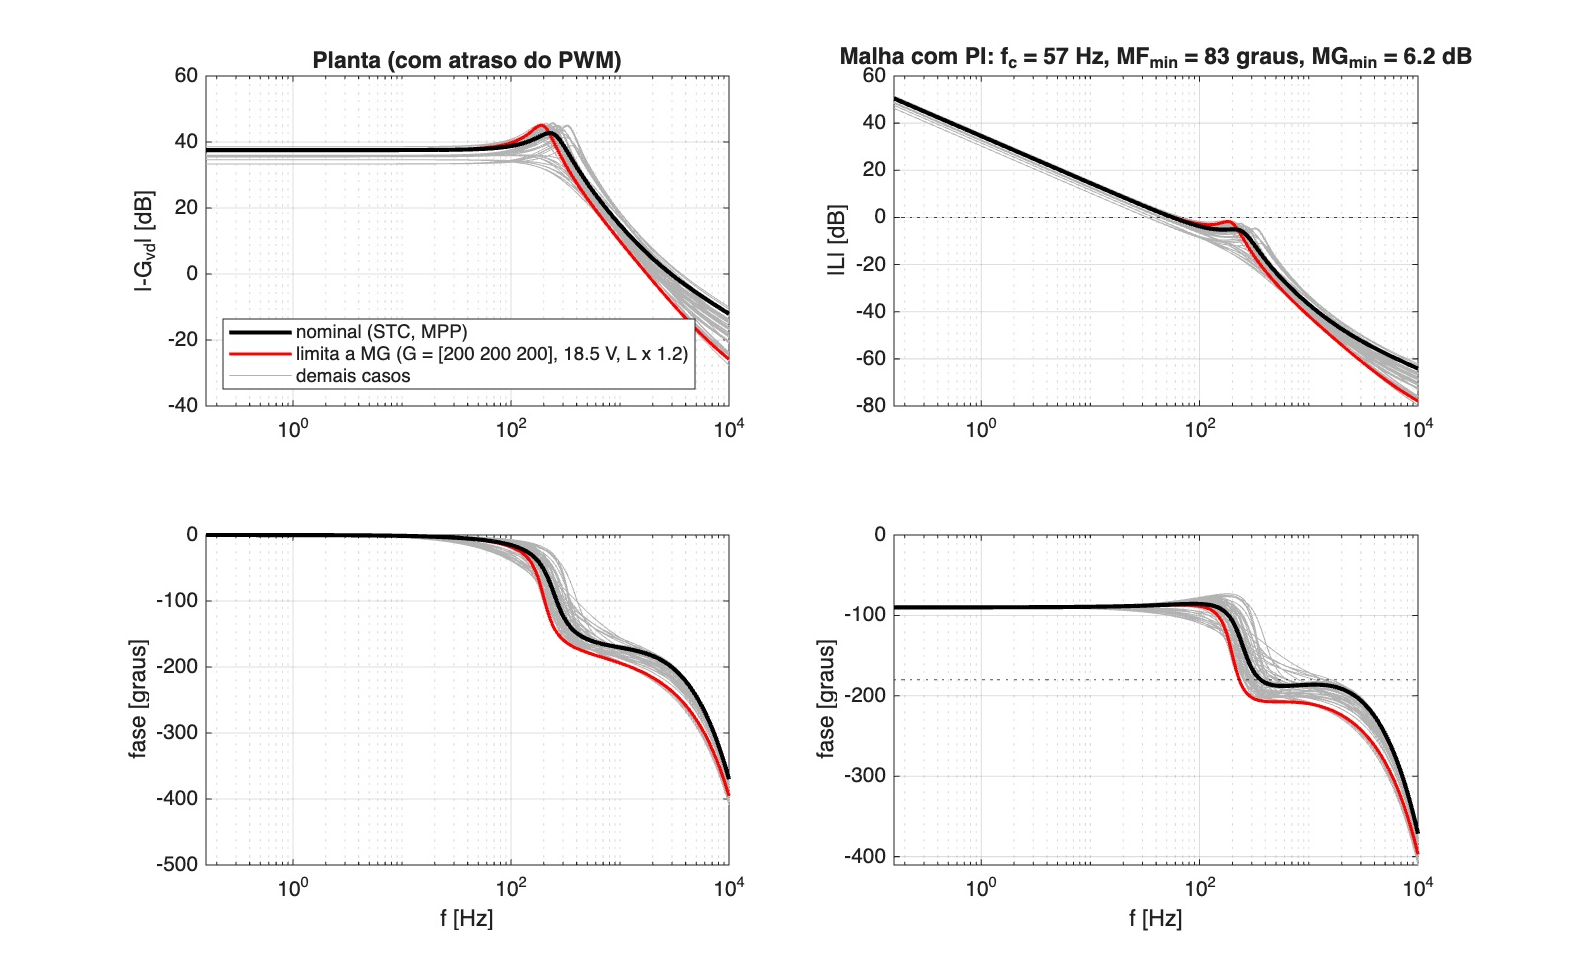
\includegraphics[width=0.95\linewidth]{e4_bode.pdf}
\caption{E4. Bode da planta e do ganho de malha com o PI. Preto: caso nominal; vermelho: o caso que limita a MG; cinza: os demais.}
\label{fig:e4bode}
\end{figure}

\begin{figure}[htbp]
\centering
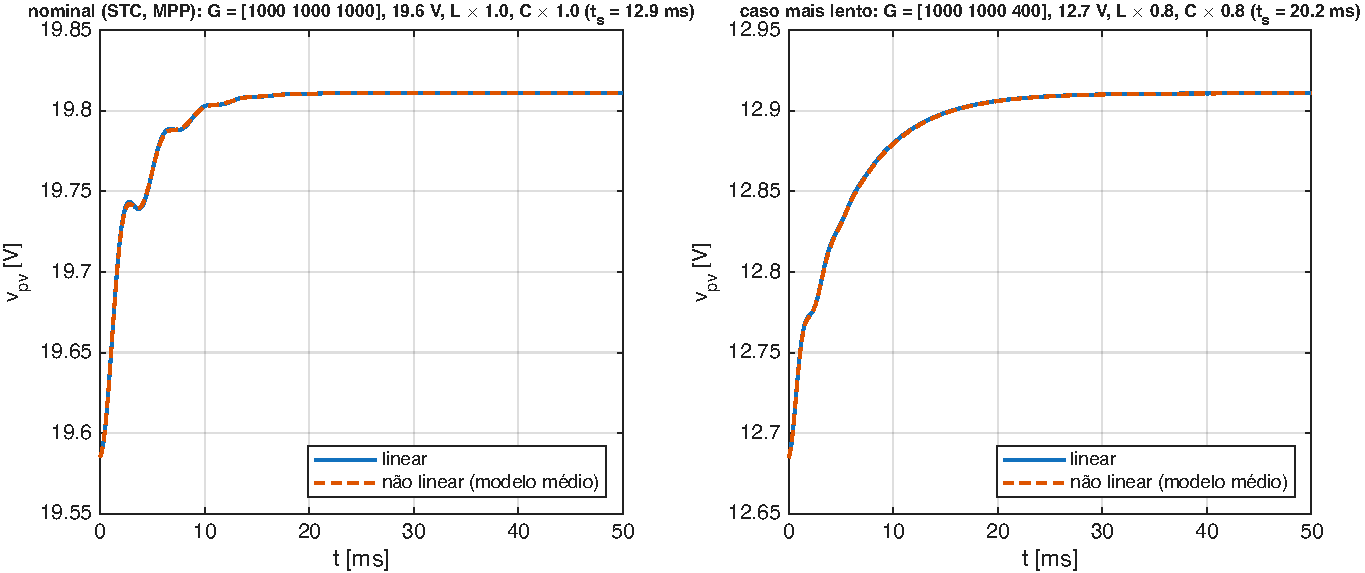
\includegraphics[width=0.9\linewidth]{e4_degrau.pdf}
\caption{E4. Degrau de $\Vref$: modelo linear (usado no projeto) contra o modelo m\'edio n\~ao linear.}
\label{fig:e4degrau}
\end{figure}

\subsection{A lei de controle com satura\c{c}\~ao}

\codigointeiro{controle/lei_pi.m}{PI de tens\~ao com satura\c{c}\~ao e anti-windup.}{lst:leipi}

\begin{logica}
\begin{enumerate}
\item $d=K_p(\text{err}+\xi/T_i)$, saturado em $[D_{min},D_{max}]=[0{,}02;\,0{,}95]$.
\item \textbf{Anti-windup:} com $d$ saturado, o integrador para se o erro empurrar o comando ainda mais para fora da faixa.
 Sem isso, $\xi$ cresceria sem limite e a malha demoraria a sair da satura\c{c}\~ao.
\item O argumento \texttt{modo} permite congelar a l\'ogica de satura\c{c}\~ao; \'e usado nos jacobianos por diferen\c{c}as finitas, para o
 passo n\~ao atravessar a descontinuidade.
\item A mesma fun\c{c}\~ao serve \`a simula\c{c}\~ao din\^amica e \`a quase-est\'atica: as duas usam exatamente o mesmo controle.
\end{enumerate}
\end{logica}

\section{Algoritmos de MPPT}\label{sec:mppt}

Arquivos: \arq{mppt/config_mppt.m}, \arq{mppt_po.m}, \arq{mppt_inc.m}, \arq{mppt_pso.m}, \arq{mppt_fixo.m},
\arq{rastrear_estatico.m}. Os tr\^es algoritmos t\^em a mesma interface,
\texttt{[Vref, e] = alg(V, I, e, cfg)}: recebem a tens\~ao e a corrente m\'edias do \'ultimo per\'iodo $\Ta$,
guardam o estado em \texttt{e} (vazio na primeira chamada) e devolvem a pr\'oxima tens\~ao de refer\^encia. Isso permite
trocar um pelo outro sem mudar a simula\c{c}\~ao.

\subsection{Perturba e Observa (P\&O)}

O P\&O \'e uma subida de encosta na curva $P(V)$. A cada per\'iodo, a refer\^encia anda um passo $\delta$. Se a pot\^encia
subiu, continua no mesmo sentido; se caiu, inverte.

\begin{figure}[htbp]
\centering
\begin{tikzpicture}
  \node[bloco,minimum width=2.8cm] (m) at (0,0) {Mede $V$, $I$\\{\scriptsize $P=V\cdot I$}};
  \node[bloco,diamond,aspect=2.2,inner sep=1pt,draw=amarelo!80!black,fill=amarelo!10] (d) at (4.3,0) {{\scriptsize $P<P_{ant}$?}};
  \node[aviso,minimum width=2.8cm] (inv) at (4.3,-2.4) {inverte a dire\c{c}\~ao\\{\scriptsize $dir\leftarrow-dir$}};
  \node[bloco,minimum width=3.4cm] (st) at (8.8,0) {$\Vref\leftarrow\Vref+dir\cdot\delta$\\{\scriptsize limita \`a faixa permitida}};
  \node[bloco,minimum width=2.6cm] (sv) at (13.0,0) {guarda\\{\scriptsize $P_{ant}=P$}};
  \draw[seta] (m) -- (d);
  \draw[seta] (d) -- node[rot,above]{n\~ao} (st);
  \draw[seta] (d) -- node[rot,right]{sim} (inv);
  \draw[seta] (inv.east) -| (st.south);
  \draw[seta] (st) -- (sv);
  \draw[seta] (sv.north) -- ++(0,1.3) -| node[rot,above,pos=0.25]{pr\'oximo per\'iodo $\Ta$} (m.north);
\end{tikzpicture}
\caption{L\'ogica do P\&O em cada per\'iodo $\Ta$.}
\label{fig:po}
\end{figure}

\begin{itemize}
\item \textbf{Vantagem:} simples e r\'apido.
\item \textbf{Oscila no MPP:} nunca para. Perto do pico fica alternando entre $V_{mp}-\delta$, $V_{mp}$ e $V_{mp}+\delta$, o que custa um pouco
 de energia ($\sim$0,1\,\% em STC no E5).
\item \textbf{Preso em pico local:} s\'o v\^e a inclina\c{c}\~ao local. Partindo de perto de $V_{oc}$, para no primeiro pico que encontra.
\end{itemize}

\codigointeiro{mppt/mppt_po.m}{Perturba e Observa.}{lst:po}

\begin{logica}
\begin{enumerate}
\item Na primeira chamada n\~ao h\'a pot\^encia anterior: o estado come\c{c}a em $V_{\mathrm{ref},0}=0{,}85V_{oc}$, descendo ($dir=-1$), pois o MPP est\'a \`a esquerda de $V_{oc}$.
\item Nas seguintes: se \texttt{P < e.Pant}, o \'ultimo passo foi no sentido errado e \texttt{e.dir} inverte. Depois guarda \texttt{P}.
\item D\'a o passo \texttt{e.Vref + e.dir*cfg.delta} e limita \`a faixa permitida. Ao bater num limite, a dire\c{c}\~ao passa a apontar para dentro, evitando uma trava
 te\'orica (refer\^encia saturada e pot\^encia constante, sem nunca inverter).
\end{enumerate}
\end{logica}

\subsection{Condut\^ancia Incremental (InC)}

No MPP, $dP/dV=0$. Como $P=VI$, isso d\'a $I+V\,dI/dV=0$, ou $dI/dV=-I/V$. Define-se
\begin{equation}
s=\frac{dI}{dV}+\frac{I}{V}=\frac{1}{V}\,\frac{dP}{dV}
\end{equation}
\begin{itemize}
\item $s>0$: est\'a \`a esquerda do MPP, aumenta a tens\~ao;
\item $s<0$: est\'a \`a direita do MPP, diminui a tens\~ao;
\item $|s|<\varepsilon$: est\'a no MPP, mant\'em a refer\^encia.
\end{itemize}
Por isso o InC n\~ao oscila, ao contr\'ario do P\&O. Como ele, s\'o enxerga a inclina\c{c}\~ao local e tamb\'em para num pico local.

\begin{figure}[htbp]
\centering
\begin{tikzpicture}
  \node[bloco,minimum width=3.0cm] (m) at (0,0) {$dV=V-V_{ant}$\\{\scriptsize $dI=I-I_{ant}$}};
  \node[bloco,diamond,aspect=2.2,inner sep=1pt,draw=amarelo!80!black,fill=amarelo!10] (d1) at (4.8,0) {{\scriptsize passo comandado}\\{\scriptsize foi zero?}};
  \node[bloco,minimum width=4.8cm] (luz) at (4.8,-2.7) {\textbf{refer\^encia mantida:} $|dI|>\epsilon_I$?\\{\scriptsize sobe se $dI>0$, desce se $dI<0$}};
  \node[bloco,minimum width=3.4cm] (s) at (10.2,0) {$s=dI/dV+I/V$};
  \node[bloco,minimum width=4.4cm] (r) at (10.2,-2.7) {se $|s|>\varepsilon$:\\{\scriptsize $\Vref\leftarrow\Vref+\mathrm{sign}(s)\,\delta$}};
  \draw[seta] (m) -- (d1);
  \draw[seta] (d1) -- node[rot,above]{n\~ao} (s);
  \draw[seta] (d1) -- node[rot,right]{sim} (luz);
  \draw[seta] (s) -- (r);
\end{tikzpicture}
\caption{L\'ogica do InC. O ramo \'e escolhido pelo passo \emph{comandado}, n\~ao pelo $dV$ medido.}
\label{fig:inc}
\end{figure}

\codigointeiro{mppt/mppt_inc.m}{Condut\^ancia Incremental.}{lst:inc}

\begin{logica}
\begin{enumerate}
\item Primeira chamada: d\'a um passo para ter dois pontos e poder calcular $dI/dV$.
\item $V\le0$ (capacitor descarregado na partida): $I/V$ n\~ao existe; sobe a tens\~ao.
\item \textbf{Refer\^encia mantida} (\texttt{e.dVref == 0}): se a corrente mudou mais que $\epsilon_I$ (0,2\,\% de $I_{sc}$), foi a irradi\^ancia: mais luz desloca o MPP para
 a direita, ent\~ao sobe a tens\~ao; menos luz, desce. O ramo \'e decidido pelo passo \emph{comandado}, pois em simula\c{c}\~ao din\^amica uma refer\^encia mantida ainda gera $dV$ de $10^{-5}$ a $10^{-3}$\,V, e dividir $dI$ por isso daria um $s$ enorme e aleat\'orio.
\item \textbf{Caso normal:} calcula $s$; se $|s|>\varepsilon$ anda $\delta$ no sentido de $\mathrm{sign}(s)$.
\end{enumerate}
\end{logica}

\textbf{Escolha de $\varepsilon$ (D14).} Um passo $\delta$ muda $s$ em cerca de $|ds/dV|\,\delta$. O ponto da grade mais pr\'oximo do MPP est\'a a no m\'aximo
$\delta/2$ dele, ent\~ao $|s|$ ali \'e no m\'aximo metade desse salto; $\varepsilon$ tem de ser pelo menos isso, ou o InC nunca para. Com
$\varepsilon=0{,}002$\,S (valor inicial) isso nunca acontecia, pois o salto medido era de 0,09 a 0,10\,S, e o InC oscilava como P\&O. O c\'odigo
calcula $\varepsilon=\tfrac12|ds/dV|\,\delta$ da curva de STC (ver \texttt{config\_mppt}).

\subsection{Enxame de part\'iculas (PSO)}

Cada part\'icula \'e uma tens\~ao candidata $x$. O conversor s\'o consegue impor uma tens\~ao por vez; ent\~ao as part\'iculas s\~ao
avaliadas \textbf{uma por per\'iodo $\Ta$}. Depois que as $N$ foram medidas, o enxame se move:
\begin{equation}\label{eq:pso}
v\leftarrow w\,v+c_1r_1\,(p_{best}-x)+c_2r_2\,(g_{best}-x),\qquad x\leftarrow x+v
\end{equation}
\begin{center}\small
\begin{tabularx}{\textwidth}{@{}l>{\raggedright\arraybackslash}Xl@{}}
\toprule
Termo & Significado & Valor \\ \midrule
$w\,v$ & In\'ercia: continua andando no sentido em que ia & $w=0{,}4$ \\
$c_1r_1(p_{best}-x)$ & Mem\'oria pr\'opria: volta ao melhor ponto que \emph{esta} part\'icula achou & $c_1=1{,}2$ \\
$c_2r_2(g_{best}-x)$ & Mem\'oria do enxame: vai ao melhor ponto que \emph{qualquer} part\'icula achou & $c_2=2{,}0$ \\
$r_1,r_2$ & Sorteios em $[0,1]$ & \texttt{RandStream} pr\'oprio \\
\bottomrule
\end{tabularx}
\end{center}

\begin{figure}[htbp]
\centering
\begin{tikzpicture}
  \node[bloco,minimum width=3.0cm] (a) at (0,0) {Aplica a part\'icula $k$\\{\scriptsize (um per\'iodo $\Ta$)}};
  \node[bloco,minimum width=3.2cm] (b) at (4.8,0) {Mede $P$ e atualiza\\{\scriptsize $p_{best}$ e $g_{best}$}};
  \node[bloco,diamond,aspect=2.2,inner sep=1pt,draw=amarelo!80!black,fill=amarelo!10] (c) at (9.8,0) {{\scriptsize todas as $N$}\\{\scriptsize medidas?}};
  \node[bloco,minimum width=3.0cm] (d) at (9.8,-2.7) {Move o enxame\\{\scriptsize eq.~(\ref{eq:pso})}};
  \node[bloco,diamond,aspect=2.2,inner sep=1pt,draw=amarelo!80!black,fill=amarelo!10] (e) at (4.8,-2.7) {{\scriptsize convergiu?}};
  \node[dest,minimum width=3.4cm] (f) at (0,-2.7) {Fixa $\Vref=g_{best}$\\{\scriptsize monitora a pot\^encia}};
  \node[aviso,minimum width=3.4cm] (g) at (0,-5.2) {Se $|\Delta P|>10\,\%$:\\{\scriptsize reinicia a busca}};
  \draw[seta] (a) -- (b);
  \draw[seta] (b) -- (c);
  \draw[seta] (c) -- node[rot,right]{sim} (d);
  \draw[seta] (c.north) -- ++(0,0.9) -| node[rot,above,pos=0.25]{n\~ao: pr\'oxima part\'icula} (a.north);
  \draw[seta] (d) -- (e);
  \draw[seta] (e) -- node[rot,above]{sim} (f);
  \draw[seta] (f) -- (g);
  \draw[seta] (e.north) -- ++(0,0.65) -| node[rot,above,pos=0.2]{n\~ao: nova rodada} (a.south);
  \draw[seta] (g.west) -- ++(-0.8,0) |- node[rot,left,pos=0.25]{reinicia} (a.west);
\end{tikzpicture}
\caption{M\'aquina de estados do PSO. Reiniciar significa voltar \`as posi\c{c}\~oes iniciais, com uma nova semente.}
\label{fig:pso}
\end{figure}

\codigointeiro{mppt/mppt_pso.m}{PSO com avalia\c{c}\~ao sequencial.}{lst:pso}

\begin{logica}
\begin{enumerate}
\item \textbf{Primeira chamada:} \texttt{iniciar} cria o estado (part\'iculas em \texttt{cfg.x0}, paradas, sem mem\'oria; gerador pr\'oprio com semente \texttt{seed + nReinicios}) e aplica a part\'icula 1.
\item \textbf{Convergido:} a primeira medi\c{c}\~ao vira a pot\^encia de refer\^encia (\texttt{Pconv}); se depois $|P-P_{conv}|>10\,\%\cdot\max(P_{conv},P_{min})$, a curva P-V mudou e a busca recome\c{c}a.
\item \textbf{Em busca:} a medi\c{c}\~ao \'e da part\'icula \texttt{k} (aplicada no per\'iodo anterior): atualiza \texttt{pbest} e \texttt{gbest}.
\item Quando todas as $N$ foram medidas, move o enxame (eq.~\ref{eq:pso}) com \texttt{rand(e.rs,\ldots)} e limita \`a faixa.
\item Para (\texttt{convergido}) se todas estiverem a menos de \texttt{tolV} do \texttt{gbest} ou se \texttt{iter >= maxIter}; ent\~ao a refer\^encia fica no \texttt{gbest}.
\end{enumerate}
\end{logica}

\textbf{Posi\c{c}\~oes iniciais (D14).} Com $N_{sub}$ diodos de bypass, os m\'aximos locais ficam perto de m\'ultiplos de $V_{mp}/N_{sub}$ (cada subm\'odulo ativo a mais soma
$\sim$ uma tens\~ao de MPP de subm\'odulo; Patel e Agarwal, 2008). O c\'odigo p\~oe uma part\'icula em cada $k\,V_{mp}/N_{sub}$ ($k=1,\dots,N_{sub}$) mais uma em
$0{,}9V_{oc}$: $N=N_{sub}+1=4$ part\'iculas. Antes, com part\'iculas espa\c{c}adas linearmente, o PSO ca\'ia no pico local em cerca de $1/3$ das sementes no padr\~ao $[1\ 0{,}6\ 0{,}3]$.

\textbf{Limita\c{c}\~oes declaradas} (vers\~ao b\'asica, de prop\'osito; ver D17): entre rein\'icios a tens\~ao fica parada no \texttt{gbest}, mas o $V_{mp}$ real deriva com a temperatura
($\sim0{,}4$\,\%/K); qualquer mudan\c{c}a de $\sim10$\,\% na pot\^encia dispara uma busca completa, mesmo que o pico global n\~ao tenha mudado de lugar; durante a busca n\~ao h\'a
teste de rein\'icio, e sob rampas r\'apidas as mem\'orias ficam velhas.

\subsection{Configura\c{c}\~ao comum}

\codigo{mppt/config_mppt.m}{44}{63}{par\^ametros do PSO: in\'ercia, atra\c{c}\~oes, part\'iculas iniciais e crit\'erios de converg\^encia e rein\'icio.}{lst:cfgpso}

\begin{center}\small
\begin{tabularx}{\textwidth}{@{}lp{3.6cm}X@{}}
\toprule
Par\^ametro & Valor & Motivo \\ \midrule
$V_{\mathrm{ref},0}$ & $0{,}85V_{oc}$ & O conversor liga com o painel quase em aberto \\
Faixa de $\Vref$ & $0{,}10V_{oc}$ a $0{,}95V_{oc}$ & Abaixo de 10\,\% a pot\^encia \'e quase nula; acima de 95\,\% o painel est\'a quase em aberto \\
Passo $\delta$ (P\&O, InC) & $0{,}01V_{oc}$ & Ajustado no E6 \\
$\varepsilon$ do InC & $\tfrac12|ds/dV|\,\delta$ & Ver acima \\
$\epsilon_I$ do InC & $0{,}002\,I_{sc}$ & Distingue mudan\c{c}a de luz de ru\'ido \\
\texttt{tolV}, \texttt{maxIter} (PSO) & $0{,}01V_{oc}$, 15 & Crit\'erio de converg\^encia \\
Limiar de rein\'icio & 10\,\% (piso 2\,\% de $P_{mp}$) & Sem o piso, no amanhecer o PSO reiniciaria sem parar \\
\bottomrule
\end{tabularx}
\end{center}

\subsection{Rastreamento est\'atico (E5)}

\arq{rastrear_estatico} isola o algoritmo da din\^amica do conversor. Sup\~oe que a malha de tens\~ao assenta dentro de um per\'iodo $\Ta$ (D13): a tens\~ao do painel \'e exatamente a
refer\^encia pedida e a corrente vem direto da curva est\'atica $I(V)$.

\codigointeiro{mppt/rastrear_estatico.m}{o la\c{c}o do rastreamento est\'atico.}{lst:rastrear}

\begin{logica}
A cada passo: resolve o painel em $V$ (com \emph{warm start}), registra $V$ e $P=VI$, e chama o algoritmo para obter o pr\'oximo $V$. Nada de EDO.
\end{logica}

O PSO usa 10 sementes por padr\~ao de sombra. A efici\^encia \'e $\eta=P_{rastreada}/P_{pico\ global}$:

\begin{resultado}
\small\centering
\begin{tabular}{@{}lccc@{}}
\toprule
Padr\~ao de irradi\^ancia & P\&O & InC & PSO (10 sementes) \\ \midrule
{[1 1 1]} (sem sombra) & 99,9\,\% & 99,97\,\% & 100,0\,\% \\
{[1 0,5 0,5]} & 99,9\,\% & 99,98\,\% & 100,0\,\% \\
{[1 0,3 0,3]} & 99,9\,\% & 100,0\,\% & 100,0\,\% \\
{[1 1 0,4]} & \textbf{67,4\,\%} & \textbf{67,6\,\%} & 99,99 a 100\,\% \\
{[1 0,6 0,3]} & \textbf{79,0\,\%} & \textbf{79,2\,\%} & 99,99 a 100\,\% \\
{[0,8 0,8 0,2]} & \textbf{42,3\,\%} & \textbf{42,2\,\%} & 99,99 a 100\,\% \\
\bottomrule
\end{tabular}
\end{resultado}

Sem sombra, ou com sombra em que o pico global \'e o mais pr\'oximo de $V_{oc}$ ([1 0,5 0,5] e [1 0,3 0,3]), os tr\^es acham o m\'aximo. Quando o global fica abaixo do local mais
perto de $V_{oc}$, P\&O e InC ficam presos e perdem de 21\,\% at\'e 58\,\%. O PSO acha o global em todas as 10 sementes de todos os padr\~oes. O pre\c{c}o \'e o tempo: de 24 a 61
per\'iodos para convergir, contra 1 a 7.

\section{Simula\c{c}\~ao: din\^amica, quase-est\'atica e or\'aculo}\label{sec:sim}

Arquivos: \arq{simulacao/sim_dinamica.m}, \arq{sim_quase_estatica.m}, \arq{oraculo_pmax.m}, \arq{oraculo_com_cache.m}. O sistema tem escalas
de tempo muito diferentes e simular tudo no detalhe m\'aximo \'e invi\'avel. A solu\c{c}\~ao foi uma \textbf{hierarquia de modelos}, cada um usado onde cabe.

\subsection{As escalas de tempo}

\begin{center}\small
\begin{tabular}{@{}ll@{}}
\toprule
Fen\^omeno & Escala de tempo \\ \midrule
Chaveamento do conversor & 50\,$\mu$s ($f_s=20$\,kHz) \\
Resson\^ancia LC & $\sim$4\,ms (240\,Hz) \\
La\c{c}o do PI (acomoda\c{c}\~ao) & $\sim$20\,ms \\
Per\'iodo do MPPT $\Ta$ & 31\,ms \\
T\'ermico do painel & $\sim$7\,min \\
Dia & 13\,h de sol \\
\bottomrule
\end{tabular}
\end{center}

O t\'ermico \'e milhares de vezes mais lento que o MPPT, e o MPPT \'e mais lento que o PI. Essa separa\c{c}\~ao permite os modelos reduzidos.

\subsection{A hierarquia de modelos}

\begin{figure}[htbp]
\centering
\begin{tikzpicture}
  \node[bloco,minimum width=4.4cm,minimum height=1.7cm] (ch) at (0,0) {\textbf{Chaveado}\\{\scriptsize Euler, $T_s/200$}\\{\scriptsize 1 a 2\,s de CPU por 6\,ms}};
  \node[ctrl,minimum width=4.4cm,minimum height=1.7cm] (me) at (5.4,0) {\textbf{M\'edio din\^amico}\\{\scriptsize EDO de 4 estados, \texttt{ode15s}}\\{\scriptsize 1 a 2,5\,s de CPU por s}};
  \node[dest,minimum width=4.4cm,minimum height=1.7cm] (qe) at (10.8,0) {\textbf{Quase-est\'atico}\\{\scriptsize regime a cada $\Ta$}\\{\scriptsize $\sim$65\,s de CPU por hora}};
  \draw[seta] (ch) -- node[rot,above]{valida (E3)} (me);
  \draw[seta] (me) -- node[rot,above]{valida (D16)} (qe);
  \node[rot,anchor=north,text width=4.2cm,align=center] at (0,-1.1) {s\'o ms};
  \node[rot,anchor=north,text width=4.2cm,align=center] at (5.4,-1.1) {transit\'orios, E6b};
  \node[rot,anchor=north,text width=4.2cm,align=center] at (10.8,-1.1) {EN 50530 e o dia inteiro (E6, E7, E8)};
\end{tikzpicture}
\caption{Cada modelo mais simples \'e conferido contra o mais detalhado, no intervalo em que ambos rodam.}
\label{fig:hierarquia}
\end{figure}

\subsection{Simula\c{c}\~ao din\^amica}

\textbf{Estado.} $x=[\vpv;\,i_L;\,\xi;\,T]$: tens\~ao do capacitor de entrada, corrente do indutor, integral do erro do PI e temperatura das c\'elulas. A corrente do painel
$I$ \emph{n\~ao} \'e estado: o painel n\~ao tem din\^amica pr\'opria nessa escala, e $I$ \'e a solu\c{c}\~ao das equa\c{c}\~oes alg\'ebricas do m\'odulo (Cap\'itulo~\ref{sec:sombra}) para a tens\~ao
$\vpv$ do momento. O \texttt{ode15s} integra a EDO reduzida $\dot x=f(x,I(x))$.

\begin{atencao}[: por que EDO reduzida e n\~ao DAE (D15)]
A formula\c{c}\~ao original era uma DAE com matriz de massa singular, como em \arq{sim_medio_aberta}. Ela falhou em 9 de 36 casos de teste, nos degraus grandes do PSO sob sombra: o
\texttt{ode15s} reaproveita o jacobiano e a condut\^ancia dos diodos varia exponencialmente ($10^{-2}$ a $10^{2}$\,S). A EDO reduzida, com o painel resolvido por Newton a cada
avalia\c{c}\~ao, teve 0 falhas em 36 casos e efici\^encias iguais em 4 d\'igitos. O pre\c{c}o \'e ficar 2 a 4 vezes mais lenta.
\end{atencao}

\begin{figure}[htbp]
\centering
\begin{tikzpicture}[node distance=0.6cm]
  \node[bloco,minimum width=4.3cm] (p1) at (0,0) {\textbf{1.} Or\'aculo no in\'icio\\{\scriptsize $P_{g0}$ com $G$ e $T$ de agora}};
  \node[bloco,minimum width=4.3cm] (p2) at (5.3,0) {\textbf{2.} Integra a EDO\\{\scriptsize \texttt{ode15s}, $t_0$ a $t_0+\Ta$, $\Vref$ fixo}};
  \node[bloco,minimum width=4.3cm] (p3) at (10.6,0) {\textbf{3.} Corrente do painel\\{\scriptsize Newton nos pontos; soma $E$}};
  \node[bloco,minimum width=4.3cm] (p4) at (10.6,-2.2) {\textbf{4.} Mede $V$ e $I$\\{\scriptsize m\'edia dos \'ultimos 20\,\% de $\Ta$}};
  \node[bloco,minimum width=4.3cm] (p5) at (5.3,-2.2) {\textbf{5.} Or\'aculo no fim\\{\scriptsize $E_g\mathrel{+}=\frac{P_{g0}+P_{g1}}{2}\Ta$}};
  \node[ctrl,minimum width=4.3cm] (p6) at (0,-2.2) {\textbf{6.} MPPT\\{\scriptsize recebe $V,I$; devolve novo $\Vref$}};
  \draw[seta] (p1) -- (p2);
  \draw[seta] (p2) -- (p3);
  \draw[seta] (p3) -- (p4);
  \draw[seta] (p4) -- (p5);
  \draw[seta] (p5) -- (p6);
  \draw[seta] (p6) -- node[rot,left]{pr\'oximo per\'iodo} (p1);
\end{tikzpicture}
\caption{O la\c{c}o de \texttt{sim\_dinamica}, repetido a cada $\Ta$. No fim, $\eta=E/E_g$.}
\label{fig:laco_sim}
\end{figure}

\codigo{simulacao/sim_dinamica.m}{132}{193}{o la\c{c}o amostrado: um intervalo $\Ta$ por itera\c{c}\~ao.}{lst:dinlaco}

\begin{logica}
\begin{enumerate}
\item \texttt{t0}, \texttt{t1}: in\'icio e fim do per\'iodo. \texttt{oraculo\_com\_cache} avalia $P_{g0}$ na ponta inicial ($G$ lida $10^{-9}\Ta$ \emph{dentro} do intervalo: um degrau de $G$ na fronteira conta para o per\'iodo certo).
\item \texttt{ode15s(f, [t0 t1], x, opts)}: integra com $\Vref$ constante (segurador de ordem zero), passando o jacobiano analítico.
\item P\'os-processamento: para cada ponto aceito, resolve o painel com \emph{warm start} (aqui os pontos est\~ao em ordem, ent\~ao \'e seguro) e soma $E=\int \vpv I\,dt$ por trap\'ezio.
\item \texttt{media\_janela}: m\'edia de $V$ e $I$ nos \'ultimos 20\,\% de $\Ta$, esperando o PI acomodar (Femia) e filtrando a oscila\c{c}\~ao residual.
\item Or\'aculo na ponta final: $E_g\mathrel{+}=\frac{P_{g0}+P_{g1}}{2}\Ta$.
\item \texttt{lei\_pi} e \texttt{verifica\_ccm} registram $d$ e se o conversor estava em CCM; por fim o MPPT devolve o novo \texttt{Vref}.
\end{enumerate}
\end{logica}

\codigo{simulacao/sim_dinamica.m}{224}{260}{lado direito da EDO: PI, conversor, t\'ermico e bloqueio do diodo.}{lst:dinrhs}

\begin{logica}
\texttt{derivadas} monta $[\dot{\vpv};\dot i_L;\dot\xi;\dot T]$: \texttt{lei\_pi} d\'a $d$ e $\dot\xi$; \texttt{conversor\_medio\_rhs} d\'a $\dot{\vpv}$ e $\dot i_L$; \texttt{termico\_dTdt} d\'a $\dot T$ (com $G$ m\'edio dos
subm\'odulos e a pot\^encia el\'etrica $\vpv I$ saindo do m\'odulo). O diodo bloqueia corrente reversa: se $i_L\le0$ e a derivada aponta para baixo, \'e zerada. \texttt{rhs} s\'o resolve o painel em $\vpv$ e chama \texttt{derivadas}.
\end{logica}

\textbf{Cuidados num\'ericos.}
\begin{itemize}
\item \textbf{Sem \emph{warm start} no lado direito}, de prop\'osito: o \texttt{ode15s} avalia fora de ordem e em passos que depois rejeita; guardar a \'ultima solu\c{c}\~ao poderia dar resultados que dependem dessa ordem.
\item \textbf{Jacobiano pela regra da cadeia:} $\partial f/\partial x=\partial f/\partial x|_I+\partial f/\partial I\cdot\partial I/\partial x$. $dI/dv$ e $dI/dT$ v\^em de deriva\c{c}\~ao impl\'icita do res\'iduo do painel com o jacobiano anal\'itico, mais preciso que diferen\c{c}as finitas perto dos joelhos do bypass.
\item \textbf{Descontinuidades} (satura\c{c}\~ao do PI, anti-windup, bloqueio do diodo): no jacobiano, o modo do PI e o estado do diodo s\~ao decididos uma vez e congelados nas avalia\c{c}\~oes perturbadas. N\~ao h\'a fun\c{c}\~oes de evento: o \texttt{ode15s} atravessa a descontinuidade rejeitando passos.
\item \textbf{Passo m\'aximo} $\Ta/20$: v\'arios pontos na janela de medida e menor erro do trap\'ezio.
\item \textbf{Pr\'e-condi\c{c}\~ao:} come\c{c}a com $G>0$; com $G=0$ o conversor n\~ao tem equil\'ibrio e a partida \'e recusada (\texttt{sim\_dinamica:inicioInviavel}).
\item \textbf{Condi\c{c}\~ao inicial:} m\'odulo em equil\'ibrio t\'ermico com o conversor desligado; integrador do PI no valor que d\'a exatamente o $d$ de equil\'ibrio (partida sem tranco).
\end{itemize}

\subsection{Or\'aculo do m\'aximo global}

A efici\^encia do MPPT \'e $\eta=E/E_g$, onde $E_g$ \'e a energia do pico global. Um MPPT preso num pico local deve aparecer com $\eta<1$.

\codigointeiro{simulacao/oraculo_pmax.m}{pot\^encia m\'axima global do painel.}{lst:oraculo}

\begin{logica}
\begin{enumerate}
\item \textbf{Varredura grossa} da curva P-V (150 pontos): descobre em que pico est\'a o m\'aximo global. Um otimizador local sozinho poderia parar no outro.
\item \textbf{Refinamento com \texttt{fminbnd}} entre os vizinhos do melhor ponto da grade: dentro desse intervalo $P(V)$ tem um s\'o m\'aximo.
\item De noite ($\max G<1$) devolve $P_g=0$. O refinamento nunca devolve menos que o melhor ponto da grade.
\end{enumerate}
\end{logica}

\codigointeiro{simulacao/oraculo_com_cache.m}{o or\'aculo s\'o recalcula se $G$ ou $T$ mudaram.}{lst:cache}

\subsection{Simula\c{c}\~ao quase-est\'atica}

Em cada $\Ta$, trata-se o sistema como em \textbf{regime permanente}: a tens\~ao do painel j\'a \'e igual a $\Vref$ e a pot\^encia \'e $P=\Vref\cdot I(\Vref)$ durante o per\'iodo todo. N\~ao h\'a EDO
el\'etrica para integrar.

\codigo{simulacao/sim_quase_estatica.m}{142}{222}{o la\c{c}o do modelo quase-est\'atico.}{lst:qelaco}

\begin{logica}
\begin{enumerate}
\item \textbf{Ponta inicial:} resolve o painel em \texttt{Vref} com $G$ e $T$ do in\'icio; o diodo impede corrente negativa (\texttt{Ia = max(Ia,0)}).
\item \textbf{Or\'aculo:} se \texttt{passoOr == 1} avalia nas duas pontas; sen\~ao, no in\'icio de cada bloco, avalia \emph{uma vez} no ponto m\'edio do bloco e segura (ver abaixo).
\item \textbf{T\'ermico:} um passo de Euler expl\'icito de tamanho $\Ta$, \texttt{Tb = T + Ta*termico\_dTdt(...)}. A pot\^encia el\'etrica sai do m\'odulo e n\~ao vira calor.
\item \textbf{Ponta final:} resolve o painel em \texttt{Vref} com $G$ e $T$ do fim.
\item \textbf{Energia:} $E\mathrel{+}=(P_a+P_b)/2\cdot\Ta$ (trap\'ezio, igual \`a din\^amica) e $E_g\mathrel{+}=P_g\Ta$.
\item \textbf{Bateria:} \texttt{potencia\_saida} usa \arq{equilibrio_conversor} para obter $P_{out}$ com perdas e classifica o ponto: CCM, DCM, invi\'avel ou sem corrente.
\item O MPPT recebe (\texttt{Vref}, \texttt{Ib}) e escolhe o pr\'oximo \texttt{Vref}.
\end{enumerate}
\end{logica}

\textbf{Op\c{c}\~oes.} \texttt{op.termico} (obrigat\'oria: com ou sem aquecimento), \texttt{op.perdas} (conversor com ou sem perdas), \texttt{op.dt\_oraculo}, \texttt{op.t\_ini} e \texttt{op.n\_log} (guarda as s\'eries s\'o a cada
$n$ per\'iodos, para economizar mem\'oria). As duas primeiras permitem a \textbf{abla\c{c}\~ao} do E7: ligar e desligar cada efeito e ver quanto ele pesa.

\textbf{Or\'aculo em blocos (D16).} O or\'aculo \'e a parte cara. Com \texttt{dt\_oraculo}$=\Ta$ custa $\sim$2500\,s de CPU por hora simulada; com 1\,s custa $\sim$65\,s. Para isso os per\'iodos s\~ao
agrupados em blocos de $\mathrm{round}(1\text{ s}/\Ta)$ per\'iodos e o or\'aculo \'e avaliado \textbf{uma vez por bloco, no ponto m\'edio}, e segurado. Numa rampa de $G$ o erro de primeira ordem se
cancela (o que falta numa metade sobra na outra), restando $\sim h^3/24\,|P_g''|$ por bloco de dura\c{c}\~ao $h$; segurar o valor do in\'icio dar\'ia erro $\sim h^2/2\,|P_g'|$, isto \'e, um atraso.
Com $dt=60$\,s o custo cai para $\sim$20\,s por hora, mas o or\'aculo atrasa nas rampas ($\eta\approx1{,}02$ numa rampa de $\sim0{,}5$\,W/m$^2$/s): por isso o valor de 1\,s.

\subsection{Validade do quase-est\'atico contra a din\^amica (D16)}

O que o quase-est\'atico ignora \'e a energia do transit\'orio depois de cada degrau de $\Vref$. O teste \texttt{test\_quase\_estatica} mede isso contra \texttt{sim\_dinamica}:

\begin{resultado}
\small\centering
\begin{tabular}{@{}ll@{}}
\toprule
Algoritmo & Erro de energia do quase-est\'atico \\ \midrule
P\&O e InC & $\le0{,}4$\,\% (cerca de $+0{,}1$\,\%) \\
PSO buscando o tempo todo (janela de 4\,s com rein\'icio) & $-1{,}1$\,\% \\
PSO numa janela t\'ipica de 20\,s (busca de 1 a 2\,s e depois segura o $g_{best}$) & cerca de $-0{,}3$\,\% \\
\bottomrule
\end{tabular}
\end{resultado}

O sinal negativo para o PSO tem causa f\'isica. Depois de um degrau grande de $\Vref$, o transit\'orio do PI passa por tens\~oes \emph{entre} as part\'iculas, perto do pico, com mais pot\^encia
que nas pontas; o quase-est\'atico s\'o conta a pot\^encia em $\Vref$. Logo o erro \'e \textbf{conservador contra o PSO}: o resultado do PSO no E7 \'e, se algo, um pouco pior que o real.

\section{Cen\'arios: EN 50530 e o dia em Florian\'opolis}\label{sec:cenarios}

Arquivos: \arq{cenarios/cenario_constante.m}, \arq{perfil_en50530.m}, \arq{dia_florianopolis.m}, \arq{aplicar_sombras.m}, \arq{baixar_pvgis.m},
\arq{data/en50530_rampas.csv}, \arq{data/clima/pvgis_floripa_2020.csv}. Todo cen\'ario \'e uma \emph{struct} com quatro campos, chamados do mesmo jeito pelos simuladores:
\texttt{cen.G(t)} (vetor $1\times N_{sub}$ com a irradi\^ancia de cada subm\'odulo), \texttt{cen.Tamb(t)}, \texttt{cen.vw(t)} (vento) e \texttt{cen.t\_fim}. Isso permite trocar o cen\'ario sem mudar a simula\c{c}\~ao.

\subsection{Cen\'ario constante}

\texttt{cenario\_constante(G, Tamb, vw, t\_fim)} devolve sempre os mesmos valores. \'E usado em testes e em experimentos curtos, como o E5.

\subsection{Perfil din\^amico da EN 50530}

A EN 50530 \'e a norma que define como medir a efici\^encia din\^amica de um MPPT. Ela aplica ao inversor uma sequ\^encia de rampas trapezoidais de irradi\^ancia, de lentas
(0,5\,W/m$^2$/s) a r\'apidas (100\,W/m$^2$/s). A irradi\^ancia \'e \emph{uniforme}: a norma testa o MPPT sem sombreamento parcial.

\textbf{A fonte (D5).} O texto da norma (CENELEC) \'e pago e n\~ao foi consultado. As tabelas B.2, B.3 e B.4 foram transcritas do relat\'orio de ensaio T\"UV Rheinland
n.$^\circ$ CN21VE2D 001 (tabela 4.4, ``Dynamic MPPT Efficiency'', p.~15 e 16). Os valores conferem aritmeticamente com as dura\c{c}\~oes impressas:
dura\c{c}\~ao $=$ repeti\c{c}\~oes $\cdot(2\,\text{rampa}+2\,\text{patamar})+$ espera. Uma inconsist\^encia foi encontrada e documentada no CSV: na B.4 o relat\'orio imprime rampa de 980\,s, mas
$(100-10)/0{,}1=900$\,s, e o c\'odigo calcula a rampa pela inclina\c{c}\~ao.

\begin{center}\small
\begin{tabular}{@{}lll@{}}
\toprule
Sequ\^encia & Faixa de $G$ [W/m$^2$] & Inclina\c{c}\~oes [W/m$^2$/s] \\ \midrule
B.2 & 100 a 500 & 0,5 / 1 / 2 / 3 / 5 / 7 / 10 / 14 / 20 / 30 / 50 \\
B.3 & 300 a 1000 & 10 / 14 / 20 / 30 / 50 / 100 \\
B.4 & 10 a 100 & 0,1 \\
\bottomrule
\end{tabular}
\end{center}

Patamares de 10\,s (30\,s na B.4), espera de 300\,s no in\'icio de cada linha e de 1 a 10 repeti\c{c}\~oes; dura\c{c}\~ao total de cerca de 7\,h.

\begin{figure}[htbp]
\centering
\begin{tikzpicture}[x=0.55cm,y=0.9cm]
  \draw[->,thick,cinza] (0,0) -- (14.5,0) node[right,font=\scriptsize]{$t$};
  \draw[->,thick,cinza] (0,0) -- (0,3.2) node[above,font=\scriptsize]{$G$};
  \draw[very thick,azul] (0,0.6) -- (2,0.6) -- (4,2.6) -- (6,2.6) -- (8,0.6) -- (10,0.6) -- (12,2.6) -- (14,2.6);
  \node[rot] at (1,0.25) {espera};
  \node[rot] at (3,1.9) {rampa};
  \node[rot] at (5,3.0) {patamar alto};
  \node[rot] at (7,1.9) {rampa};
  \node[rot] at (9,0.25) {patamar baixo};
  \node[rot,left] at (0,0.6) {$G_{baixo}$};
  \node[rot,left] at (0,2.6) {$G_{alto}$};
\end{tikzpicture}
\caption{Estrutura de cada linha da tabela: espera em $G_{baixo}$ e depois um n\'umero de trap\'ezios (rampa, patamar alto, rampa, patamar baixo).}
\label{fig:trapezio}
\end{figure}

\codigointeiro{cenarios/perfil_en50530.m}{monta $G(t)$ como lista de pontos interpolada linearmente.}{lst:en50530}

\begin{logica}
\begin{enumerate}
\item L\^e o CSV (\texttt{readtable} com coment\'arios \texttt{\%}) e valida: espera $>1$\,ms, patamar $>0$, $G_{alto}>G_{baixo}$.
\item Para cada linha: o degrau inicial leva 1\,ms (o interpolador exige instantes estritamente crescentes), depois a espera; a rampa dura $(G_{alto}-G_{baixo})/\text{inclina\c{c}\~ao}$.
\item Cada repeti\c{c}\~ao adiciona 4 pontos (sobe, patamar alto, desce, patamar baixo).
\item \texttt{griddedInterpolant} interpola linearmente; $G$ \'e a mesma em todos os subm\'odulos. $T_{amb}=25\,^\circ$C e vento 1\,m/s, porque a norma separa o MPPT do efeito t\'ermico.
\end{enumerate}
\end{logica}

\subsection{O dia em Florian\'opolis}

Para o dia real o trabalho usa dados do \textbf{PVGIS} (base PVGIS-SARAH3), no ponto de lat.\ $-27{,}595^\circ$, lon.\ $-48{,}548^\circ$ e altitude 34\,m. O m\'odulo est\'a inclinado a $27^\circ$ e
voltado para o norte. O dia escolhido foi \textbf{26/01/2020} (c\'eu claro de ver\~ao). \texttt{dia\_florianopolis} faz:

\begin{enumerate}
\item L\^e o CSV do PVGIS (tem cabe\c{c}alho e rodap\'e de texto: s\'o as linhas que come\c{c}am com a data \texttt{yyyyMMdd:HHmm} s\~ao dados).
\item Converte de UTC para a hora local (UTC$-3$), para $t=0$ ser a meia-noite local.
\item Usa as colunas $G(i)$ (irradi\^ancia no plano), $T_{2m}$ (temperatura do ar) e $WS_{10m}$ (vento a 10\,m).
\item Interpola as amostras hor\'arias de forma suave (\texttt{pchip}).
\item Converte o vento de 10\,m para o vento junto ao m\'odulo ($\sim$2\,m) pela lei de pot\^encia de expoente $1/7$: fator $(2/10)^{1/7}\approx0{,}79$.
\item Define a janela de sol: instantes com $G>5$\,W/m$^2$.
\end{enumerate}

\subsection{Nuvens e sombras sint\'eticas (D6)}

Os dados hor\'arios n\~ao t\^em transit\'orios r\'apidos nem sombras. Por isso foram criados eventos \textbf{sint\'eticos}, declarados como tais no relat\'orio e gravados em \arq{resultados/e7_eventos.csv}.

\begin{center}\small
\begin{tabular}{@{}llllll@{}}
\toprule
Hora & Dura\c{c}\~ao & Evento & Subm\'odulo & Fator & Rampa \\ \midrule
10:30 a 10:36 & 6\,min & Nuvem & Todos & 0,4 & 20\,s \\
11:15 a 11:16:12 & 72\,s & Nuvem & Todos & 0,3 & 10\,s \\
14:00 a 14:45 & 45\,min & Sombra de poste & 3 & 0,3 & 60\,s \\
14:45 a 15:00 & 15\,min & Sombra de poste & 2 & 0,3 & 60\,s \\
15:00 a 15:30 & 30\,min & Poste (mais fraca) & 3 & 0,5 & 60\,s \\
\bottomrule
\end{tabular}
\end{center}

As duas nuvens cobrem o m\'odulo todo e testam o rastreamento sob mudan\c{c}a r\'apida de luz. A sombra de poste anda sobre o m\'odulo e cria, com um subm\'odulo sombreado, uma curva
com dois picos: o trecho em que P\&O e InC podem ficar presos e o PSO deve ganhar. Nas transi\c{c}\~oes de 60\,s os dois eventos se sobrep\~oem.

\codigointeiro{cenarios/aplicar_sombras.m}{multiplica $G$ por um fator com rampas lineares.}{lst:sombras}

\begin{logica}
A vari\'avel \texttt{a} \'e um trap\'ezio no tempo: rampa de subida (de 0 a 1 em \texttt{rampa\_s} segundos a partir de \texttt{t\_ini}) menos rampa de descida (que come\c{c}a em \texttt{t\_fim}).
O fator aplicado \'e $f=1-(1-\text{fator})\,a$. Com \texttt{sub = 0} afeta todos os subm\'odulos (nuvem); com \texttt{sub = j}, s\'o o subm\'odulo $j$ (poste). \texttt{Gbase} \'e avaliada uma \'unica vez por chamada.
\end{logica}

\section{Experimentos e resultados}\label{sec:resultados}

Cada experimento \'e um script \texttt{matlab/experimentos/expNN\_*.m} que grava tabelas em \arq{resultados/} (CSV) e figuras em \arq{relatorio/figs/}. Esta se\c{c}\~ao resume o que cada um
mede e conclui.

\subsection{Vis\~ao geral}

\begin{center}\small
\begin{tabularx}{\textwidth}{@{}l>{\raggedright\arraybackslash}X>{\raggedright\arraybackslash}Xc@{}}
\toprule
Exp. & O que mede & Resultado principal & Cap. \\ \midrule
E1 & Valida\c{c}\~ao do painel e identificabilidade & Erro de $V_{oc}$ 0,03\,\%; $\gamma_P$ $-0{,}363$ contra $-0{,}4$\,\%/K; efici\^encia em 200\,W/m$^2$ entre 93,1 e 94,8\,\% & \ref{sec:extracao} \\
E2 & Curvas I-V e P-V sob sombra & At\'e 3 picos; o global pode estar em qualquer um & \ref{sec:sombra} \\
E3 & Chaveado contra m\'edio & Concordam em CCM; separam-se em DCM & \ref{sec:conversor} \\
E4 & Bode, margens e degrau do PI & $f_c=56{,}6$\,Hz, MG m\'inima 6,2\,dB, $t_s=20{,}2$\,ms, $\Ta=31$\,ms & \ref{sec:controle} \\
E5 & MPPT est\'atico com sombra & P\&O/InC chegam a 42\,\%; PSO $\ge99{,}99$\,\% & \ref{sec:mppt} \\
E6 & MPPT na EN 50530 & P\&O 99,9\,\%, InC 99,6\,\%, PSO 98,6\,\% & \ref{sec:e6} \\
E6b & Trecho da EN 50530 no modelo din\^amico & Din\^amico e quase-est\'atico concordam & \ref{sec:e6b} \\
E7 & Dia real com sombras e abla\c{c}\~ao & PSO 98,7\,\%; t\'ermico pesa 9\,\%, perdas pesam 11\,\% & \ref{sec:e7} \\
E8 & Modelo anterior contra completo & O anterior superestima a energia em 21,9\,\% & \ref{sec:e8} \\
\bottomrule
\end{tabularx}
\end{center}

\subsection{E6: MPPT na EN 50530 (sem sombra)}\label{sec:e6}

O perfil de cerca de 7\,h \'e simulado no quase-est\'atico, com $T=25\,^\circ$C fixa e or\'aculo a cada 1\,s. A efici\^encia \'e $\eta=E/E_g$, com $E_g=352{,}95$\,Wh dispon\'iveis. O passo $\delta$ do P\&O e
do InC \'e o compromisso cl\'assico: $\delta$ grande segue rampas r\'apidas mas oscila mais em torno do MPP; $\delta$ pequeno oscila pouco mas fica para tr\'as. Por isso varreu-se $\delta=0{,}5$; $1$ e
$2$\,\% de $V_{oc}$ ($\varepsilon$ do InC \'e reescalado junto).

\begin{resultado}
\small\centering
\begin{tabular}{@{}llccc@{}}
\toprule
Algoritmo & $\delta$ [\% $V_{oc}$] & $\eta$ & Energia na bateria [Wh] & Rein\'icios \\ \midrule
P\&O & 0,5 & 99,92\,\% & 323,85 & --- \\
P\&O & 1 & 99,90\,\% & 323,77 & --- \\
P\&O & 2 & 99,62\,\% & 322,92 & --- \\
InC & 0,5 & 98,79\,\% & 319,93 & --- \\
InC & 1 & 99,16\,\% & 321,17 & --- \\
InC & 2 & 99,58\,\% & 322,64 & --- \\
PSO & --- & 98,62\,\% & 319,67 & 2182 \\
\bottomrule
\end{tabular}
\end{resultado}

\textbf{Como ler.} Sem sombra, P\&O e InC t\^em de 99,6\,\% a 99,9\,\% e o PSO \'e 1,3 ponto pior. O motivo: o PSO reinicia a busca a cada rampa (2182 rein\'icios no perfil) e, a cada busca, passa v\'arios per\'iodos avaliando
part\'iculas longe do pico. Quando a luz s\'o varia de forma uniforme n\~ao h\'a pico global escondido, e esse custo n\~ao compensa. O conversor fica em DCM em cerca de 30\,\% do tempo, por causa das irradi\^ancias baixas do perfil (10 a 100\,W/m$^2$).

\subsection{E6b: confer\^encia no modelo din\^amico}\label{sec:e6b}

Um trecho curto da sequ\^encia B.3 ($G$ de 300 a 1000\,W/m$^2$, 50\,W/m$^2$/s, 2 trap\'ezios, 106\,s) roda tamb\'em na \texttt{sim\_dinamica}, com a espera inicial encurtada para 10\,s:

\begin{resultado}
\small\centering
\begin{tabular}{@{}lcc@{}}
\toprule
Algoritmo & $\eta$ din\^amico & $\eta$ quase-est\'atico \\ \midrule
P\&O & 99,88\,\% & 99,88\,\% \\
InC & 99,49\,\% & 99,49\,\% \\
PSO & 97,79\,\% & 97,62\,\% \\
\bottomrule
\end{tabular}
\end{resultado}

Os dois modelos concordam em P\&O e InC, e para o PSO o quase-est\'atico fica 0,2 ponto abaixo, no sentido conservador do Cap\'itulo~\ref{sec:sim}. Os ``dentes'' do PSO na figura s\~ao as buscas.

\begin{figure}[htbp]
\centering
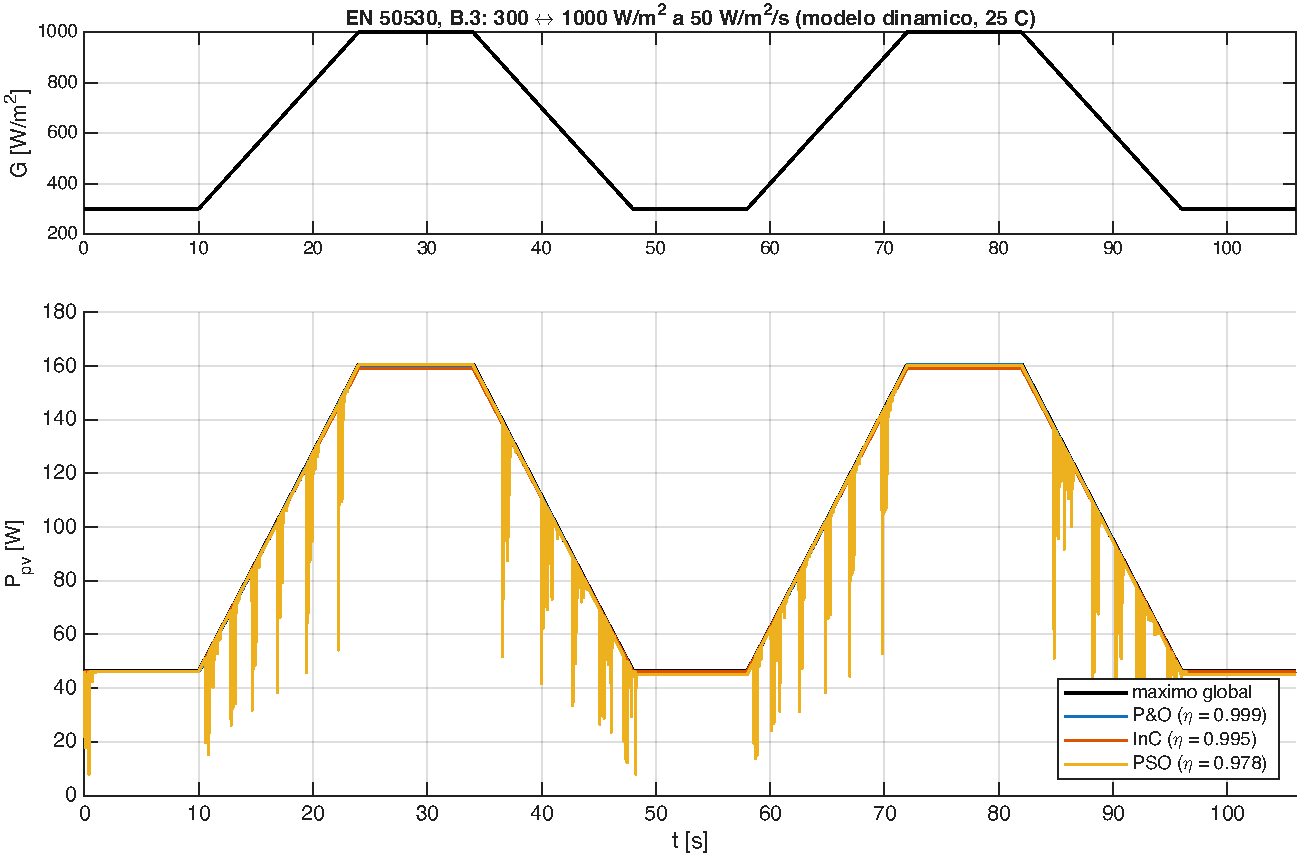
\includegraphics[width=0.95\linewidth]{e6_dinamico.pdf}
\caption{E6b. Como cada algoritmo segue as rampas no modelo din\^amico.}
\label{fig:e6b}
\end{figure}

\subsection{E7: dia em Florian\'opolis com sombras e abla\c{c}\~ao}\label{sec:e7}

O dia 26/01/2020 com os eventos sint\'eticos, no modelo completo, com 3 algoritmos $\times$ 3 variantes (completo, sem t\'ermico, sem perdas) = 9 rodadas de 9 a 23\,min de CPU.

\begin{resultado}
\small\centering
\begin{tabular}{@{}llcccc@{}}
\toprule
Variante & Algoritmo & $E_{pv}$ [Wh] & $E_{bat}$ [Wh] & $\eta$ & $\Delta E_{bat}$ \\ \midrule
Completo & P\&O & 1018,5 & 913,4 & 95,7\,\% & --- \\
Completo & InC & 997,6 & 896,5 & 93,8\,\% & --- \\
Completo & PSO & 1050,8 & \textbf{941,7} & \textbf{98,7\,\%} & --- \\
\midrule
Sem t\'ermico (25\,$^\circ$C) & P\&O & 1108,8 & 993,7 & 95,6\,\% & $+8{,}8$\,\% \\
Sem t\'ermico (25\,$^\circ$C) & InC & 1091,2 & 976,8 & 94,1\,\% & $+9{,}0$\,\% \\
Sem t\'ermico (25\,$^\circ$C) & PSO & 1143,7 & 1020,8 & 98,6\,\% & $+8{,}4$\,\% \\
\midrule
Sem perdas & P\&O & 1018,5 & 1018,5 & 95,7\,\% & $+11{,}5$\,\% \\
Sem perdas & InC & 997,6 & 997,6 & 93,8\,\% & $+11{,}3$\,\% \\
Sem perdas & PSO & 1050,8 & 1050,8 & 98,7\,\% & $+11{,}6$\,\% \\
\bottomrule
\end{tabular}
\end{resultado}

\begin{itemize}
\item \textbf{O PSO ganha na sombra.} Na sombra de poste (14:00 a 15:00), P\&O e InC ficam no pico de alta tens\~ao, com cerca de metade da pot\^encia dispon\'ivel; o PSO reinicia, acha o global e o segue. A energia n\~ao captada, de $\sim$1064\,Wh
 dispon\'iveis, \'e de 13,8\,Wh para o PSO (1,3\,\%), 45,7\,Wh para o P\&O (4,3\,\%) e 66,2\,Wh para o InC (6,2\,\%).
\item \textbf{Na bateria}, o PSO entrega 28,3\,Wh (3,1\,\%) a mais que o P\&O e 45,2\,Wh (5,0\,\%) a mais que o InC.
\item \textbf{O aquecimento pesa 9\,\%.} O m\'odulo chega a 55,6--55,7\,$^\circ$C; ignor\'a-lo aumenta a energia dispon\'ivel em 9,0\,\% e a da bateria em 8,4 a 9,0\,\%.
\item \textbf{As perdas do conversor pesam 11\,\%.} Ignor\'a-las aumenta a energia na bateria em 11,3 a 11,6\,\%; a efici\^encia m\'edia do conversor no dia \'e de 89,6 a 89,9\,\%; o conversor fica em DCM em $\sim$13\,\% dos per\'iodos.
\item \textbf{Os dois efeitos s\~ao maiores que a diferen\c{c}a entre o melhor e o pior algoritmo} (5,0\,\%) e n\~ao mudam o ordenamento: um modelo isot\'ermico ou sem perdas erra a energia mais do que a escolha do algoritmo.
\item O PSO reiniciou 104 vezes no dia. Os eventos de sombra reduzem a energia dispon\'ivel de cerca de 1138\,Wh (o mesmo dia sem eventos) para 1064\,Wh.
\end{itemize}

\begin{figure}[htbp]
\centering
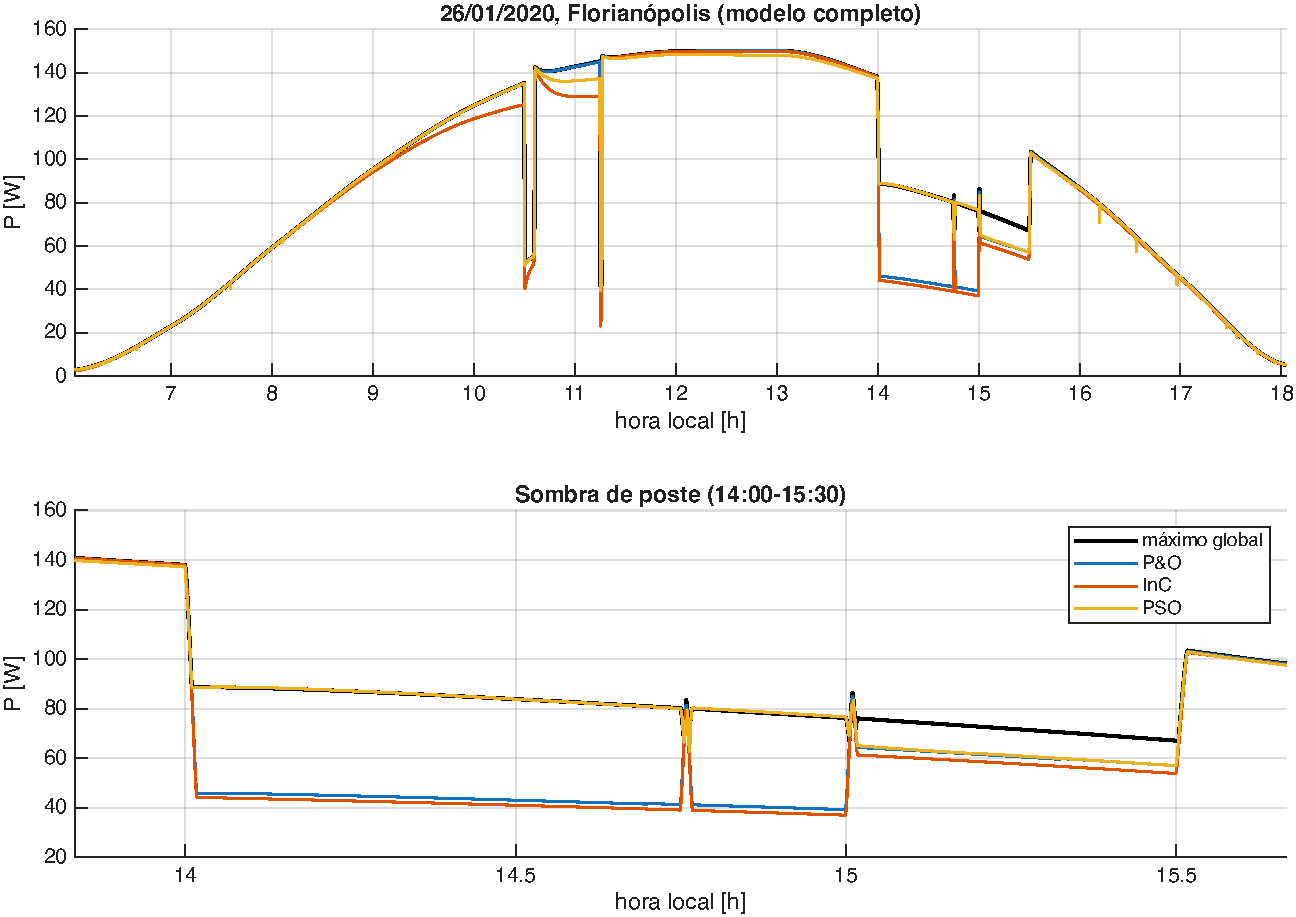
\includegraphics[width=0.95\linewidth]{e7_dia.pdf}
\caption{E7. Pot\^encia ao longo do dia (modelo completo). Preto: m\'aximo global (or\'aculo); demais: pot\^encia extra\'ida por P\&O, InC e PSO. Embaixo, o detalhe da sombra de poste.}
\label{fig:e7}
\end{figure}

\subsubsection{Tr\^es limita\c{c}\~oes que s\'o o dia real revela (D17)}

Ficaram documentadas como resultado, sem alterar os algoritmos (corrigi-las exigiria rodar E6 e E7 de novo, horas de CPU):
\begin{enumerate}
\item \textbf{O PSO n\~ao acompanha a deriva t\'ermica.} Depois de convergir ele fica parado no $g_{best}$. Quando o m\'odulo esquenta de 43 para 53\,$^\circ$C depois da nuvem das 10:30, o $V_{mp}$ cai, mas o PSO s\'o reinicia se a pot\^encia mudar mais de 10\,\%: fica 3 a 4\,\% abaixo do m\'aximo.
\item \textbf{O InC ``congela''.} S\'o sai do lugar se $\Delta I>0{,}2\,\%\,I_{sc}$ por amostra ($\sim$18\,mA); varia\c{c}\~oes lentas de luz n\~ao chegam a isso.
\item \textbf{O PSO erra o pico global com sombra fraca e m\'odulo quente.} Com $[1\ 1\ 0{,}5]\cdot656$\,W/m$^2$ a 44\,$^\circ$C, as part\'iculas iniciais erram o pico global (11,6\,V) e o enxame converge no local (18,9\,V).
\end{enumerate}

\subsection{E8: o trabalho anterior contra o modelo completo}\label{sec:e8}

O mesmo dia, sem os eventos de sombra, com P\&O nos dois casos e o mesmo PI. O modelo ``anterior'' usa 1 diodo, conversor ideal e c\'elulas a 25\,$^\circ$C; o ``completo'', 2 diodos, perdas e t\'ermico.

\begin{resultado}
\small\centering
\begin{tabular}{@{}lccc@{}}
\toprule
Modelo & $E_{pv}$ [Wh] & $E_{bat}$ [Wh] & $T_{m\acute ax}$ [$^\circ$C] \\ \midrule
Anterior (1 diodo, ideal, 25\,$^\circ$C) & 1238,4 & 1238,4 & 25,0 \\
Completo (2 diodos, perdas, t\'ermico) & 1137,2 & 1015,8 & 55,6 \\
\bottomrule
\end{tabular}
\end{resultado}

O anterior \textbf{superestima a energia na bateria em 21,9\,\%} ($1238{,}4/1015{,}8=1{,}219$). A diferen\c{c}a se decomp\~oe de forma multiplicativa: as perdas do conversor respondem por
$1137{,}2/1015{,}8=1{,}120$ ($+12$\,\%); o resto, $1238{,}4/1137{,}2=1{,}089$ ($+9$\,\%), re\'une a temperatura e a troca de 2 para 1 diodo. Como s\'o a temperatura j\'a aumenta a energia
dispon\'ivel em 9,0\,\% no E7, a contribui\c{c}\~ao do modelo de 1 diodo \'e praticamente nula, coerente com o E1 (os dois modelos s\~ao ajustados aos mesmos pontos e diferem pouco perto de STC, onde est\'a quase toda a energia de um dia de ver\~ao).
\textbf{O erro n\~ao estava no n\'umero de diodos, mas no que ficou fora do modelo.}

\begin{atencao}[: ressalva]
O E8 \'e uma \emph{reconstru\c{c}\~ao}: o modelo ``anterior'' usa o ajuste de 1 diodo bem posto deste trabalho, para isolar o efeito das simplifica\c{c}\~oes. A extra\c{c}\~ao original do trabalho anterior dava $\sim$121\,W com o MPP perto de 15\,V, contra 160\,W
em 19,6\,V aqui. Esse erro de par\^ametros se somaria \`as simplifica\c{c}\~oes e n\~ao est\'a nos 21,9\,\%.
\end{atencao}

\section{Testes, simplifica\c{c}\~ao do c\'odigo e verifica\c{c}\~ao}\label{sec:testes}

\subsection{O harness de testes}

\arq{matlab/run_tests.m} chama \texttt{setup\_path} (que p\~oe as pastas do projeto no \emph{path}) e roda \texttt{runtests} em \arq{matlab/tests/}; falha se algum teste falhar. S\~ao 14 arquivos
com \texttt{matlab.unittest} e \textbf{78 testes} (eram 81 antes da simplifica\c{c}\~ao e 80 depois dela; os 2 testes do LM sa\'iram junto com ele). Cada teste prova uma propriedade f\'isica ou um contrato, e o coment\'ario diz de onde vem o valor esperado.

\codigo{tests/test_conversor.m}{11}{37}{tr\^es testes do conversor: ganho ideal, balan\c{c}o de energia e derivadas nulas no equil\'ibrio.}{lst:teste}

\begin{logica}
\begin{enumerate}
\item \texttt{test\_ganho\_ideal}: sem perdas o ganho do buck-boost \'e $d/(1-d)=V_{bat}/\vpv$ e $\eta=1$ (f\'isica pura).
\item \texttt{test\_balanco\_de\_energia}: a pot\^encia de entrada $\vpv\ipv$ deve ser igual \`a pot\^encia na bateria mais as perdas de condu\c{c}\~ao; $P_{out}=P_{in}-P_{cond}-P_{sw}$; e $0{,}85<\eta<1$.
\item \texttt{test\_rhs\_nulo\_no\_equilibrio}: no equil\'ibrio calculado por \texttt{equilibrio\_conversor}, as derivadas de \texttt{conversor\_medio\_rhs} s\~ao nulas. Confere \emph{dois} c\'odigos diferentes entre si.
\end{enumerate}
\end{logica}

\begin{center}\small
\begin{tabularx}{\textwidth}{@{}l>{\raggedright\arraybackslash}X@{}}
\toprule
Arquivo & O que verifica \\ \midrule
\arq{test_kcl_modulo} & O res\'iduo do m\'odulo e a inclina\c{c}\~ao $dI/dV$ (deriva\c{c}\~ao impl\'icita) \\
\arq{test_extracao} & A extra\c{c}\~ao no KC200GT contra o resultado publicado de Villalva \\
\arq{test_ztp160m}, \arq{test_ztp160m_extracao} & Pontos de STC do ZTP-160M, converg\^encia dos modelos 1d e 2d, $\gamma_P$ \\
\arq{test_sombreamento} & $P_{mp}$ e $V_{mp}$ de refer\^encia, n\'umero de picos, comportamento do bypass \\
\arq{test_termico} & Calibra\c{c}\~ao pelo NMOT, efeito do vento e da extra\c{c}\~ao de eletricidade \\
\arq{test_conversor} & Balan\c{c}o de energia, derivadas nulas no equil\'ibrio, ponto invi\'avel, dimensionamento \\
\arq{test_chaveado_medio} & M\'edio contra chaveado: desvio $<0{,}5$\,\% em $v$, $<1{,}5$\,\% em $i_L$, ripple dentro de 15\,\% \\
\arq{test_linearizacao} & A planta linearizada contra \texttt{gvd\_analitico} \\
\arq{test_controle} & Margens, tempo de acomoda\c{c}\~ao, $\Ta\ge1{,}5\,t_s$, e a falha da regra $\omega_c/5$ \\
\arq{test_mppt} & Cada algoritmo em curvas conhecidas, incluindo o preso em pico local \\
\arq{test_sim_dinamica} & Energia, or\'aculo e partida da simula\c{c}\~ao din\^amica \\
\arq{test_quase_estatica} & Quase-est\'atico contra din\^amico (D16), blocos do or\'aculo e totais \\
\arq{test_cenarios} & EN 50530, convers\~ao de hora do PVGIS e eventos de sombra \\
\bottomrule
\end{tabularx}
\end{center}

Uma ideia recorrente \'e a de \textbf{regress\~ao por comparativo}: um modelo mais detalhado serve de refer\^encia para um mais simples. O m\'edio \'e conferido contra o chaveado, o quase-est\'atico contra o
din\^amico, o jacobiano anal\'itico contra diferen\c{c}as finitas e a planta num\'erica contra a anal\'itica.

\subsection{A etapa de simplifica\c{c}\~ao do c\'odigo}

Depois do trabalho conclu\'ido foi feita uma auditoria para deixar o c\'odigo mais simples, com um crit\'erio r\'igido: \textbf{nenhum n\'umero do relat\'orio pode mudar}. Como a licen\c{c}a do MATLAB estava vencendo,
os experimentos n\~ao foram rodados de novo; s\'o entraram mudan\c{c}as de risco baixo, que apenas reorganizam o c\'odigo. O processo foi: spec, plano, achados (etapa 1: modelo e experimentos; etapa 2: testes),
decis\~ao item a item, aplica\c{c}\~ao em lotes e revis\~ao independente. Os documentos est\~ao em \arq{docs/superpowers/simplificacao/}.

\textbf{Etapa 1, 9 achados de risco baixo aplicados:}
\begin{enumerate}
\item \texttt{levenberg\_marquardt} (removido depois, ver Cap\'itulo~\ref{sec:extracao}) sem o argumento opcional \texttt{opts} e a subfun\c{c}\~ao \texttt{campo}, que ningu\'em usava.
\item \texttt{curva\_pv} sem o campo de sa\'ida \texttt{c.Vj}, que ningu\'em lia.
\item \texttt{sim\_medio\_aberta} sem o argumento \texttt{max\_passo} e sem a generalidade de $G$ como fun\c{c}\~ao do tempo.
\item \texttt{sim\_chaveado} sem a sa\'ida \texttt{r.q}.
\item \texttt{projeto\_pi} sem \texttt{rel.tabela} e sem o \texttt{ts\_nom} s\'o usado para preench\^e-la (economiza 400 chamadas de \texttt{resposta\_degrau\_mf}).
\item Remo\c{c}\~ao do \texttt{mkdir} defensivo em 9 scripts de experimento, pois as pastas s\~ao versionadas.
\item Cria\c{c}\~ao de \texttt{oraculo\_com\_cache.m}, antes uma subfun\c{c}\~ao duplicada nos dois simuladores.
\item \texttt{lei\_pi} chamada uma vez, e n\~ao duas, dentro do jacobiano da \texttt{sim\_dinamica}.
\item Remo\c{c}\~ao de coment\'ario sobre uma op\c{c}\~ao (\texttt{op.V0}) que n\~ao existia no quase-est\'atico.
\end{enumerate}
O achado 10 (unificar as seis resolu\c{c}\~oes de \texttt{curva\_pv}) tem risco m\'edio: mudaria $P_{mp}$, $V_{mp}$ e $V_{oc}$ por pouco e, em cascata, $L$, $C$, o PI e todos os CSVs. N\~ao foi aplicado.

\textbf{Etapa 2 (testes).} Achados 1, 2 e 5 aplicados: um teste duplicado de \texttt{test\_conversor} foi fundido no de balan\c{c}o de energia, um campo n\~ao usado do \texttt{setupOnce} saiu, e o
\emph{setup} de um caso do ZTP-160M foi movido para o \'unico teste que o usa. Os achados 3 e 4 foram recusados, para o teste de extra\c{c}\~ao continuar autossuficiente. O teste \texttt{test\_fechada\_igual\_fzero}
foi renomeado para \texttt{test\_d\_fechado\_satisfaz\_equilibrio}, pois o nome citava um \texttt{fzero} que ele n\~ao usa.

\textbf{O que ficou de fora de prop\'osito.} A auditoria tamb\'em registrou o que \emph{n\~ao} foi mexido e por qu\^e. O \emph{setup} repetido entre arquivos de teste (2 a 5 linhas) ficou, porque uma fun\c{c}\~ao compartilhada
esconderia de onde vem cada par\^ametro, o que vai contra o estilo exigido (simples, expl\'icito, leg\'ivel por um j\'unior).

\subsection{Resultado da simplifica\c{c}\~ao}

\begin{center}\small
\begin{tabular}{@{}lrrr@{}}
\toprule
Pasta & Linhas antes & Depois & Varia\c{c}\~ao \\ \midrule
numerico & 56 & 47 & $-9$ \\
painel & 242 & 240 & $-2$ \\
termico & 35 & 35 & 0 \\
conversor & 125 & 117 & $-8$ \\
controle & 224 & 216 & $-8$ \\
mppt & 140 & 140 & 0 \\
simulacao & 324 & 315 & $-9$ \\
cenarios & 91 & 91 & 0 \\
experimentos & 480 & 466 & $-14$ \\
tests & 812 & 806 & $-6$ \\
\textbf{Total} & \textbf{2548} & \textbf{2492} & $\boldsymbol{-56}$ \\
\bottomrule
\end{tabular}
\end{center}

S\~ao linhas de c\'odigo (sem coment\'ario e sem branco). Os coment\'arios (1494 antes, 1486 depois) foram mantidos porque explicam a f\'isica. A conclus\~ao da auditoria foi que o c\'odigo j\'a estava enxuto: as
$\sim$4400 linhas totais se explicam porque 34\,\% s\~ao coment\'arios, os testes somam 806 linhas, os experimentos 466, o escopo \'e amplo e s\'o havia o MATLAB base, sem toolboxes.

\subsection{Como se verificou que nada quebrou}

\begin{itemize}
\item \textbf{Testes:} 81 de 81 antes; 81 de 81 depois da etapa 1; 80 de 80 depois da etapa 2; 78 de 78 depois de trocar o LM pelo \texttt{fsolve} (10/11/2026, ap\'os a simplifica\c{c}\~ao).
\item \textbf{\texttt{checkcode}} (o analisador do MATLAB) nos arquivos alterados: nenhum aviso, antes nem depois.
\item \textbf{Revis\~ao independente da etapa 1:} conformidade e qualidade aprovadas; as duas observa\c{c}\~oes menores, s\'o de coment\'ario, foram corrigidas.
\item \textbf{Prova de que os testes enxutos n\~ao ficaram mais fracos:} a mesma perturba\c{c}\~ao no modelo faz o teste antigo e o novo falharem. Por exemplo, apagar \texttt{- eq.Psw} em \texttt{equilibrio\_conversor.m} d\'a 1 falha no antigo e 1 no
 novo; trocar \texttt{r.E = E} por \texttt{1.02 * E} em \texttt{sim\_quase\_estatica.m} d\'a 4 falhas no antigo e 4 no novo.
\item \textbf{Refer\^encias:} nenhuma refer\^encia \'orf\~a em \texttt{matlab/}, no relat\'orio ou no README.
\end{itemize}

\begin{atencao}[: ponto fraco a declarar]
Os experimentos \textbf{n\~ao foram rodados de novo} depois da simplifica\c{c}\~ao. A garantia de que os n\'umeros n\~ao mudam vem de as mudan\c{c}as serem s\'o reorganiza\c{c}\~ao (o mesmo c\'odigo, mudado de lugar ou sem as linhas n\~ao
usadas). E6, E7 e E8 n\~ao foram reexecutados. O \texttt{git log} mostra a branch \texttt{simplificacao} j\'a mesclada (commit \texttt{3f4f1ed}).
\end{atencao}

\section{Conclus\~oes, limita\c{c}\~oes, como rodar e gloss\'ario}\label{sec:fim}

\subsection{Resposta \`a pergunta central}

\begin{resumo}
\textbf{Sob sombreamento parcial est\'atico, o P\&O pode perder de 21 a 58\,\% da pot\^encia dispon\'ivel} (efici\^encias de 79\,\% a 42\,\%), porque para no pico local; o PSO recupera praticamente tudo ($\ge99{,}99$\,\%).

Num dia real de ver\~ao em Florian\'opolis, com uma hora de sombra de poste e duas nuvens, considerando o aquecimento do m\'odulo (at\'e 55,6\,$^\circ$C) e as perdas do conversor, o P\&O deixa de captar 45,7\,Wh (4,3\,\% da energia
dispon\'ivel) e o PSO, 13,8\,Wh (1,3\,\%). Na bateria, o PSO entrega 3,1\,\% a mais que o P\&O e 5,0\,\% a mais que o InC.

A busca global tem um custo: sem sombra, no perfil EN 50530, o PSO perde 1,3 ponto de efici\^encia para o P\&O, porque reinicia a cada rampa. O PSO compensa quando h\'a sombras que deslocam o pico global, e n\~ao compensa quando o c\'eu s\'o varia de forma uniforme.
\end{resumo}

\textbf{Sobre a modelagem.} Os resultados que mais pesam na energia n\~ao v\^em dos algoritmos: ignorar o aquecimento superestima a energia em cerca de 9\,\% e ignorar as perdas do conversor, em cerca de 11\,\%; juntas, as simplifica\c{c}\~oes do trabalho anterior
d\~ao $+21{,}9$\,\%. Do lado dos m\'etodos, o trabalho mostrou que (i) o datasheet n\~ao identifica o segundo diodo e o gap precisa ser efetivo; (ii) $R_p(G)$ corrige uma perda de 26\,\% em baixa irradi\^ancia sem significado f\'isico; (iii) a DAE com matriz de massa falha em 9 de 36 casos e a EDO
reduzida resolve; e (iv) a hierarquia chaveado $\to$ m\'edio $\to$ quase-est\'atico, validada em cada degrau, permite simular as 13\,h de sol em 9 a 23\,min de CPU.

\subsection{Limita\c{c}\~oes}

\begin{itemize}
\item \textbf{Sem curvas I-V medidas.} O datasheet n\~ao as traz; a valida\c{c}\~ao do painel \'e indireta (STC, $\gamma_P$, NMOT, KC200GT), e o $\gamma_P$ do modelo ($-0{,}363$\,\%/K) fica abaixo do do datasheet ($-0{,}4$\,\%/K).
\item \textbf{Diodos de bypass: hip\'otese.} O datasheet informa a associa\c{c}\~ao ``3$\times$11'' das 33 c\'elulas, mas n\~ao quantos diodos h\'a; adotaram-se 3 subm\'odulos de 11 c\'elulas, a configura\c{c}\~ao usual.
\item \textbf{Ruptura reversa n\~ao modelada.} O bypass conduz muito antes dela, ent\~ao o efeito na curva \'e pequeno, mas o aquecimento local (\emph{hot spot}) fica fora.
\item \textbf{Temperatura uniforme.} Na realidade, um subm\'odulo sombreado fica mais frio que os outros.
\item \textbf{Bateria ideal.} A tens\~ao fixa em 12\,V n\~ao varia com o estado de carga.
\item \textbf{Sombras e nuvens sint\'eticas.} Os dados do PVGIS s\~ao hor\'arios; os resultados de energia valem para esse cen\'ario, n\~ao para um dia t\'ipico.
\item \textbf{Quase-est\'atico conservador contra o PSO}, cerca de 1\,\% enquanto ele busca; no perfil EN 50530 a efici\^encia do PSO pode estar subestimada nessa ordem.
\item \textbf{Margem de ganho apertada.} MG de 6,2\,dB no pior caso, a 0,2\,dB do requisito.
\item \textbf{DCM n\~ao modelado.} O modelo m\'edio de CCM n\~ao descreve os 13 a 32\,\% do tempo em DCM, onde as perdas de condu\c{c}\~ao s\~ao subestimadas.
\item \textbf{Perdas de cat\'alogo}, n\~ao de um prot\'otipo: a abla\c{c}\~ao mostra o tamanho do efeito, n\~ao o valor exato.
\item \textbf{A EN 50530 foi transcrita de um relat\'orio de ensaio}, n\~ao da norma; a data do relat\'orio T\"UV ainda aparece como ``s.d.'' na bibliografia (pend\^encia opcional).
\end{itemize}

\textbf{Trabalho futuro:} reverifica\c{c}\~ao peri\'odica e posi\c{c}\~oes iniciais corrigidas pela temperatura no PSO; limiar de corrente proporcional \`a irradi\^ancia no InC; passo do InC al\'em de 2\,\% de $V_{oc}$; ganho
escalonado no PI; modelo de DCM; temperatura por subm\'odulo; e valida\c{c}\~ao experimental com curvas I-V medidas do ZTP-160M.

\subsection{Como rodar}

Requer o \textbf{MATLAB} com a \textbf{Optimization Toolbox} (s\'o para o \texttt{fsolve} da extra\c{c}\~ao de par\^ametros). Testado no R2026b.

\begin{lstlisting}[language=Matlab,style=matlabcod,numbers=none]
cd matlab
run_tests                 % todos os testes
exp01_validacao_painel    % cada experimento grava em resultados/ e relatorio/figs/
\end{lstlisting}

\begin{center}\small
\begin{tabular}{@{}ll@{}}
\toprule
Experimento & Tempo aproximado de CPU \\ \midrule
\texttt{exp01} a \texttt{exp05}, \texttt{exp06b} & Minutos \\
\texttt{exp06\_en50530} & $\sim$1\,h \\
\texttt{exp07\_dia} & $\sim$2 a 3\,h (se \texttt{resultados/e7\_series.mat} existir, s\'o redesenha a figura) \\
\texttt{exp08\_baseline} & $\sim$30\,min \\
\bottomrule
\end{tabular}
\end{center}

\textbf{Rode um experimento longo de cada vez:} processos MATLAB em paralelo esgotam a mem\'oria. Os dados do PVGIS j\'a est\~ao versionados; para baix\'a-los de novo, \texttt{baixar\_pvgis(2020)}.

Para compilar os documentos:
\begin{lstlisting}[language=bash,numbers=none,basicstyle=\ttfamily\scriptsize]
cd relatorio && tectonic -X compile relatorio.tex
cd guia      && tectonic -X compile guia_implementacao.tex
cd proposta  && python3 gerar_figuras.py && tectonic -X compile proposta.tex
\end{lstlisting}

\subsection{Gloss\'ario}

{\small
\begin{longtable}{@{}p{3.6cm}p{12.4cm}@{}}
\toprule
Termo & Significado \\ \midrule \endhead
STC & Condi\c{c}\~oes padr\~ao de teste: 1000\,W/m$^2$ e 25\,$^\circ$C de c\'elula \\
NMOT & Temperatura nominal de opera\c{c}\~ao do m\'odulo: 800\,W/m$^2$, ar a 20\,$^\circ$C, vento de 1\,m/s \\
MPP / MPPT & Ponto de m\'axima pot\^encia / seu rastreamento \\
P\&O, InC, PSO & Perturba e Observa; Condut\^ancia Incremental; Otimiza\c{c}\~ao por Enxame de Part\'iculas \\
$V_{oc},I_{sc},V_{mp},I_{mp}$ & Tens\~ao de circuito aberto, corrente de curto, tens\~ao e corrente no MPP \\
Subm\'odulo & Grupo de c\'elulas em s\'erie protegido por um diodo de bypass \\
Diodo de bypass & Diodo em antiparalelo que desvia a corrente em torno de um subm\'odulo sombreado \\
Pico local e global & M\'aximos da curva P-V com sombra; o global \'e o maior \\
Or\'aculo & Fun\c{c}\~ao que calcula o m\'aximo global verdadeiro, para medir $\eta$ \\
$\eta$ MPPT & Energia rastreada dividida pela energia do m\'aximo global \\
CCM e DCM & Condu\c{c}\~ao cont\'inua e descont\'inua ($i_L$ zera a cada per\'iodo) \\
Raz\~ao c\'iclica $d$ & Fra\c{c}\~ao do per\'iodo em que a chave est\'a ligada \\
Ripple & Oscila\c{c}\~ao pico a pico de uma grandeza por causa do chaveamento \\
Margem de fase e de ganho & Folgas de estabilidade da malha; usual: MF $\ge45^\circ$ e MG $\ge6$\,dB \\
Anti-windup & Congelar o integrador do PI quando o atuador satura \\
Quase-est\'atico & Tratar conversor e PI como em regime a cada per\'iodo do MPPT \\
EDO e DAE & Equa\c{c}\~oes diferenciais ordin\'arias; diferenciais e alg\'ebricas \\
\texttt{fsolve} & Resolve sistemas n\~ao lineares $r(y)=0$ (Optimization Toolbox); aqui, por regi\~ao de confian\c{c}a \\
PVGIS & Base de dados de irradi\^ancia e clima da Comiss\~ao Europeia \\
\bottomrule
\end{longtable}}


\end{document}
